% %%%%%%%%%%%%%%%%%%%%%%%%%%%%%%%%%%%%%%%%%%%%%%%%%%%%%%%
% Please note that whilst this template provides a 
% preview of the typeset manuscript for submission, it 
% will not necessarily be the final publication layout.
%
%% Document class options: (**...** are defaults)
%  - bibtex: Uses bibtex+natbib, chicago.bst 
%  - biblatex: Uses biblatex-chicago
%      You MUST select one of the above two options, depending
%      on whether you prefer bibtex or biblatex. This template
%      contains code that uses bibtex.
%  - twocolumn: Switch to two column for main text
%  - singlespace/onehalfspace/**doublespace**: 
%         changes line spacing for main text
%  - **blind**/nonblind: Anonymises authors 
%         and affiliations, or not
%  - autowc: Automatically inserts a word count
%         after the abstract, using texcount. 
%         The abstract is ignored. 
%         NOTE THAT THIS WILL ONLY WORK IF YOU HAVE  
%         INSTALLED TEXCOUNT, AND HAVE ENABLED --shell-escape
%         OR --enable-write18. (These will work on Overleaf.)
%         If you get an error about "texcount not found", delete
%         the autowc option, and manually specify the wordcount 
%         with \totalwordcount{xxx}.
%%% autowc may cause longer compilation time. You can 
%%% disable it first while actively editing, and only
%%% enable it when you're ready to take stock and check
%%% on your work.
\documentclass[bibtex, autowc]{apsr_submission}
% \totalwordcount{500}

%% Example alternative options with everything the opposite of the above: (DO NOT USE AUTOWC WITH BIBLATEX; the word count will be greatly over-reported)
% \documentclass[biblatex,nonblind,singlespace,twocolumn]{apsr_submission}

\title{The Shadow of Deterrence: Why capable actors engage in conflict short of war}

% The custom \author command takes THREE arguments:
% #1 = Author name
% #2 = Affiliation name
% #3 = Brief author profile, or anything that you'd usually put in a \thanks. Leave blank {} if there's nothing to be said.
\author{J Andr\'{e}s Gannon}
       {University of California, San Diego}
       {J Andres Gannon is a PhD Candidate in the Department of Political Science, University of California, San Diego. Corresponding Author (jagannon@ucsd.edu).}
       
\author{Erik Gartzke}
       {University of California, San Diego}
       {Erik Gartzke is a Professor of Political Science at the University of California, San Diego. (egartzke@ucsd.edu).}
       
\author{Jon R. Lindsay}
       {University of Toronto}
       {Jon R. Lindsay is an Assistant Professor of Digital Media and Global Affairs at the University of Toronto. (jon.lindsay@utoronto.ca).}

\author{Peter Schram}
       {Vanderbilt University}
       {Peter Schram is an Assistant Professor of Political Science at Vanderbilt University. (peter.schram@vanerbilt.edu).}

%% Any other acknowledgements or author notes
\thanks{The authors wish to thank the members of the Center for Peace and Security Studies (cPASS), particularly Rex Douglass, as well as Nadiya Kostyuk, Chad Levinson, John Warden, and Christopher Whyte for thoughtful feedback. Tom Brailey, Cole Reynolds, Benjamin Smalley, and Erin Werner provided excellent research assistance. Earlier drafts of this paper were presented at the 2018 STRATCOM Deterrence Symposium and the 2018 American Political Science Association conference. This research was sponsored by Office of Naval Research Grant N00014-14-1-0071 and the Department of Defense Minerva Research Initiative. Any opinions, findings, and conclusions or recommendations expressed in this publication are those of the authors and do not necessarily reflect the view of the U.S. government. Data and code for the empirical analysis can be found at \texttt{https://github.com/CenterForPeaceAndSecurityStudies/GrayZone}}

%% These are used for the headers
\runningtitle{The Shadow of Deterrence}
\runningauthor{Gannon et al.} % 4 + Authors, Author One et al. 

%% Useful packages
\usepackage{amsmath}
\usepackage{graphicx}
\usepackage{rotating}
\usepackage{pgfplots}
\usepackage{bm}
\pgfplotsset{compat=newest}
  %% the following commands are needed for some matlab2tikz features
  \usetikzlibrary{plotmarks}
  \usetikzlibrary{arrows.meta}
  \usepgfplotslibrary{patchplots}
  \usepackage{grffile}

\graphicspath{{./figures/}}
%% If you are using a custom figure or table environment from a package and it's not getting framed, add \makeframedenv{MyFigure} in the preamble, where the custom figure environment is \begin{MyFigure}...\end{MyFigure}.
%% Currently table, table*, figure, figure*, longtable, supertabular, sidewaystable and sidewaysfigure will be automatically framed.

%% Handy for setting wide tables/figures in landscape
\usepackage{pdflscape}

%% Recent LaTeX distributions should be able to automatically convert .eps to .pdf; but if this isn't happening, try loading the epstopdf package manually
% \usepackage{epstopdf}

%%% Use \addbibresource{...} if using BibLaTeX
% \addbibresource{GrayZone.bib}

\begin{document}
%%% DO NOT REMOVE THESE LINES. For automatic word count.
%TC:ignore
\begin{frontmatter}
\begin{abstract}
Recent conflicts have increasingly occurred in the ``gray zone'' between peace and open warfare. New technologies or tactics---from cyber operations to ``little green men''---may make aggression at low intensities more attractive to challengers (cheaper/more effective). Alternatively, existing deterrence networks may force motivated challengers to act more furtively (stability-instability). These dueling ``push-pull'' logics suggest contrasting conflict dynamics impacting stability and peace. We develop a game theoretic model to analyze gray zone conflict in which deterrence success is variable, rather than dichotomous. In the model, the scope and intensity of a challenger's provocation varies inversely with the implicit credibility of the defender's deterrent threat. We find empirical support for the stability-instability logic in Russian military actions since the 1990s; Russia is more restrained, and less effective, against nations in, or closely tied to, NATO. States face inherent trade-offs between stability and military potency in limiting the risk of escalation. 
\end{abstract}
\end{frontmatter}
%%% DO NOT REMOVE THIS LINE. For automatic word count.
%TC:endignore

\section{Introduction}

\dropcap{In} the wake of the downfall of Ukrainian President Viktor Yanukovych in February 2014, the Crimean Peninsula was invaded by “little green men,” soldiers whose uniforms lacked insignia or other identifying information. The Kremlin formally annexed Crimea shortly thereafter. Protracted ground skirmishes, cyber campaigns, and ``active measures'' continue to plague Ukraine \citep{angevine_learninglessonsukraine_2019}. Russia's intervention has emerged as a paradigmatic example of a technologically novel and politically efficient form of ``hybrid warfare,'' designed to challenge the status quo without triggering a broader conflict \citep{marten_putinchoicesexplaining_2015, lanoszka_russianhybridwarfare_2016, chivvis_hybridwarrussian_2017}. Similar tactics and imagery have emerged elsewhere. For example, Chinese ``little blue men'' have been accused of eroding ``red lines'' in maritime East Asia \citep{green_counteringcoercionmaritime_2017}. According to former British Defense Secretary Michael \citet{fallon_speechdeliveredsecretary_2017}, ``That is not a Cold War. It is a grey war. Permanently teetering on the edge of outright hostility. Persistently hovering around the threshold of what we would normally consider acts of war.'' 

There is increasing concern that conventional conceptions of deterrence are inadequate to conceptualize and deal with burgeoning threats ``in the gray zone'' \citep{matisek_shadesgraydeterrence_2017}. Indeed, deterrence is typically believed to have failed if a challenger disrupts the status quo or resorts to military violence. As General \citet{dunford_gendunfordremarks_2016}, Chairman of the United States Joint Chiefs of Staff, commented, “Our traditional approach is either we’re at peace or at conflict. And I think that’s insufficient to deal with the actors that actually seek to advance their interests while avoiding our strengths.” 

Rather than repudiating deterrence, however, gray zone strategies could actually reflect efforts by challengers to sustain existing frameworks, both to avoid major war and because they share key interests in common with status quo powers. The main source of discrepancy may lie in how we have come to think about deterrence, rather than how it is practiced. Deterrence helps to determine \textit{how} a challenger disrupts, in addition to \textit{whether}. Shaping other nations' behaviors could certainly prove valuable, even in the absence of peace and a full retention of the status quo. An enemy that engages ``with one hand tied behind its back'' to avoid triggering a larger contest is not fighting as effectively. Even if the challenger resorts to force and the defender does not intervene, fear of subsequent intervention by the defender could cause the challenger to adopt a more furtive (indecisive) military strategy.

We develop a formal model to differentiate and assess two distinct causal logics for gray zone conflict, one driven by military innovation (reduced costs or more effective aggression) and the other by deterrence. We also explore their distinctive empirical implications. In our model, a challenger and defender can select from variable intensities of limited conflict or choose to resolve the crisis with a decisive war. We show that the challenger's choice varies with the level of the deterrent threat posed by the defender, the challenger's valuation for the stakes, and the challenger's costs for fighting. We then test key results of the model, finding empirical evidence that the magnitude and risk of NATO intervention shapes recent Russian uses of force. We also find some (but weaker) evidence that Russia moderates the intensity of its efforts in response to the implicit credibility of the West's deterrence posture along an East-West gradient. These outcomes suggest Russian behavior is predicted by deterrence, and not only by the logic of gray zone as military innovation. 

In the sections that follow, we first locate gray zone conflict in the broader literature on limited war (Section 2). We then analyze limited conflict using a formal model to illustrate the trade-offs that states face in deciding to enter into gray zone conflict or to go to war (Sections 3-5). Next, we assess our argument empirically, using data on Russian aggression, with an emphasis on cyber operations (Section 6). We then revisit the game theoretical results to discuss critical challenges of defense in the gray zone (Section 7). We conclude with implications of our argument (Section 8).

\section{Between Peace and War}
Despite the analytical convenience offered by conceptualizing war and peace as discrete outcomes, there is nothing new about conflict that falls ambiguously between peace and war \citep{lebow_futurewar_2010}. There is a long history of, and a vast literature on, limited war \citep{kissinger_militarypolicydefense_1955, osgood_reappraisallimitedwar_1969}, salami slicing tactics \citep{schelling_armsinfluence_1966}, low-intensity conflict \citep{turbiville_prefacefuturetrends_2002}, revolutionary war \citep{shy_revolutionarywar_1986}, military operations other than war \citep{kinross_clausewitzlowintensityconflict_2004}, covert operations and proxy wars \citep{carson_secretwarscovert_2018, orourke_covertregimechange_2018}, small wars \citep{olson_conceptsmallwars_1990}, hybrid wars \citep{lanoszka_russianhybridwarfare_2016}, frozen conflict \citep{driscoll_friendsthesebrinkmanship_2016}, and hassling \citep{schram_hasslinghowstates_2020}.

Early Cold War writings on “weakening the enemy with pricks instead of blows” \citep[186]{hart_strategyindirectapproach_1954} emphasized limited political objectives in the shadow of nuclear escalation. The Korean War seemed a then-underappreciated type of war fought to achieve political ends short of total victory with military means short of a total commitment \citep{osgood_reappraisallimitedwar_1969}. Contemporary treatments understood limited war as a conflict between actors that had the capacity to increase battlefield commitments but did not want to do so, creating a third option between major war and acquiescence \citep{brodie_morelimitedwar_1957, kissinger_strategyorganization_1957}. Strategists introduced the "stability-instability paradox" to describe how disincentives for nuclear war, or even major conventional war, encourage conflict at lower levels of intensity, or in peripheral theaters \citep{jervis_illogicamericannuclear_1984, sagan_spreadnuclearweapons_2003}. There is some threshold above which any given threat becomes too costly to be both credible and effective, and non-credibility invites challenges. As \citet[167]{snyder_balancepowerbalance_1965} observes, “nuclear technology introduced a new form of intent-perception and a new form of uncertainty — that concerning what types of military capability the opponent was likely to use and what degree of violence he was willing to risk or accept.” Similarly, \citet[598]{powell_nuclearbrinkmanshiplimited_2015} notes that “the amount of power the challenger brings to bear affects the stability of the conflict. More specifically, how much power the challenger brings to bear limits how much risk the defender can generate.” As \citet[173]{george_deterrenceforeignpolicy_1989} explain, adversaries can ``design around'' deterrence by discovering new options that offer “an opportunity for gain while minimizing the risk of an unwanted response by the defender”. This can result in serious fighting, as when Egypt “designed around” Israel’s deterrent in 1973 \citep{stein_calculationmiscalculationconventional_1989}. Even so, “designing around” remains a perverse symptom of deterrence success because the adversary chooses its challenge in an effort to avoid the anticipated retaliation of the defender \citep{lieberman_reconceptualizingdeterrencenudging_2012}.

Yet, other wars are limited not by the risk of escalation, but rather by cost concerns. During the Cold War there were numerous decolonization struggles and proxy wars in the developing world. In these “low intensity conflicts” or “small wars,” the immediate adversaries tended to be irregular or guerrilla forces rather than peer competitors \citep{galula_counterinsurgencywarfaretheory_1964, taber_warfleaclassic_1965, schultz_lowintensitywarfarechallenge_1986}. An insurgent might give all, but still not be able to give much. Guerrillas with rudimentary arsenals and limited personnel simply could not directly engage powerful security forces, and thus opted for indirect ambush and subversion as a matter of necessity. After the Cold War, as great power competition waned and the United States became embroiled in occupations abroad, there was a revival of interest in questions of counterterrorism and counterinsurgency \citep{nagl_learningeatsoup_2005, kilcullen_counterinsurgency_2010}. Yet a common theme involves the limited military capacity of at least one of the combatants. Asymmetric contests thus contrast starkly with a superpower opting to forego military effectiveness to control escalation. 

The renewal of interest in low-intensity conflict between more capable competitors represents a return to the earlier theme. A common thread in definitions of gray zone conflict is that it involves “a carefully planned campaign operating in the space between traditional diplomacy and overt military aggression” employed by challengers with grand geopolitical ambitions and potent capabilities \citep{mazarr_masteringgrayzone_2015}. A number of pundits highlight the growing diversity of technologies by which low intensity conflict can be practiced \citep{wirtz_lifegrayzone_2017}. Even sceptics of cyber warfare highlight the expanded repertoire of means available for low-intensity conflict, especially online espionage and disinformation \citep{rid_cyberwarpeace_2013, jensen_fancybearsdigital_2019}. If technological advances drive gray zone conflict, then we might expect to see Russia engaging in it as often as possible.

However, militaries have been innovating novel technologies across multiple domains, at all levels of intensity. Thus the choice to use some of these innovations, but not others, really represents a restriction, rather than an expansion, of conflict behavior. Focusing on gray zone conflict as a reduction rather than expansion of options calls into question claims about its innovative effectiveness below the threshold of war. On the contrary, the familiar logic of the stability-instability paradox may be playing out today at different, and usually lower, thresholds \citep{lindsay_coercioncyberspacestabilityinstability_2018}. In its classic formulation, nuclear deterrence paradoxically encourages peripheral conventional war. Today, the prospect of costly conventional war encourages provocation in cyberspace. The bad news about persistent conflict is thus good news about restraint. 

In the last decade of the Cold War, US Secretary of State George \citet{schultz_lowintensitywarfarechallenge_1986} offered a note of cautious optimism in this regard:
    
    \begin{quote}
        The ironic fact is, these new and elusive challenges have proliferated, in part, because of our success in deterring nuclear and conventional war. Our adversaries know they cannot prevail against us in either type of war. So they have done the logical thing: they have turned to other methods. Low-intensity warfare is their answer to our conventional and nuclear strength a flanking maneuver, in military terms.
    \end{quote}
    
Below we develop Schultz's insight to explore whether modern gray zone conflict should be viewed as similarly reassuring or newly alarming. 

\section{Theoretical Intuition}
The Euromaidan Revolution presented Russia with a new political reality: Kiev was abruptly realigning with the West. Almost as quickly, Russia set about altering this new ``status quo.''\footnote{The notion of ``status quo'' is inherently contextual, and thus subject to perspective and interpretation. Here, we treat the status quo as whatever political conditions prevail at a given point in time, regardless of past changes.} Russia's actions in Ukraine were limited and, because Russia stands to benefit from continued access to Crimea and from instability in Ukraine, politically advantageous. We refer to this behavior as ``challenging the status quo,'' or conducting ``limited challenges'' (implicitly to the status quo). In response to Russian activity, NATO increased its presence in the Black Sea, reinforced its support for capacity-building in Ukraine, and has stepped up its presence and cooperation in other countries in Eastern Europe. This has helped Ukraine in countering the Russian-sponsored separatist movement in the East of the country, and in dampening other related disruptions, such as cyber attacks.

The model we present in the next section captures these strategic dynamics. In the model, two actors, a challenger and a defender, experience a crisis. As the first move, the challenger decides whether to accept the status quo and do nothing, to conduct limited challenges, or to escalate to war. If the challenger conducts a limited challenge, the defender has an opportunity to respond with acceptance, escalation to war, or countering the challenge to the status quo with the defender's own limited conflict.\footnote{The challenge and countering-the-challenge moves here are similar to "hassling" or "containment" as defined in \citet{schram_hasslinghowstates_2020} and \citet{joseph_littlebitcheaptalk_2020} (respectively), but are broader. For example, hassling specifically degrades a challenger's future military capabilities, which "challenges" could do here.} When the challenger engages in limited activity and the defender responds with a limited response (rather than accepting or going to war), we will say that the states are engaged in a gray zone conflict. Thus, gray zone conflict occurs when militarily capable challengers intentionally limit the intensity and capacity with which they conduct military operations, and the defender engages but chooses not to escalate to a decisive war. Narrowing the scope of gray zone conflict to militarily capable actors distinguishes the phenomenon from wars limited by cost by clarifying that actors are making a choice to limit the intensity of their engagement, rather then being compelled to do so by limited capabilities. Importantly, gray zone conflict must be preferred by both sides in a contest; both actors have the capacity to escalate to a larger war, but they choose not to. Escalation must thus be mutually undesirable, meaning that gray zone conflict is an equilibrium \citep{carson_facingsavingface_2016, carson_secretwarscovert_2018}.

Our model highlights the trade-offs confronting actors when choosing varying degrees of force. An actor may forgo the most effective or decisive means for the job when these means are too costly, they are not committed enough, or when some other more appealing alternative exists. While war can accomplish an aggressor’s goals, it could also be unnecessary and inefficient if partial victories or \textit{faits accomplis} can be achieved at lower cost, or risk \citep{altman_advancingattackingstrategic_2018}. By considering these trade-offs, our model offers insight concerning two central questions related to gray zone conflict. First, why do states engage in gray zone conflict and, once they do, what explains variation in the intensity with which they pursue gray zone conflict? Second, when a defender faces the prospect of limited challenges, when does restrained behavior within the gray zone serve to benefit the defender?

Why do states engage in gray zone conflict? Challengers that attempt to alter the status quo through limited challenges must decide how aggressive the activity should be. A more intensive challenge can yield greater political gains. But the challenger faces two possible constraints into selecting limited challenges: an \textit{external deterrent constraint}, and an \textit{internal efficiency constraint}. If the \textit{external deterrent constraint} binds, the challenger is resolved, but will limit the level of force to attempt to avoid a greater war. Thus, when the deterrent constraint binds, the challenger is most reactive to the defender's willingness to go to war. Alternatively, if the \textit{internal efficiency constraint} binds, the challenger selects relatively low levels of force based on its own internal cost-benefit calculations. With the internal constraint, the challenger is most sensitive to its own valuation of the stakes versus the costs of challenging the status quo. 
 
The theoretical distinction here is subtle, but empirically consequential. When the challenger's internal efficiency constraint binds, the challenger is able to choose the scope and intensity of conflict that it believes is most efficient for accomplishing its objective. The challenger can focus on pursuing the optimal challenge without concern of provoking an escalation, effectively wasting less effort for more political effect. When the challenger's external deterrent constraint binds, by contrast, the challenger must scale back from its optimal low-level challenge in order to avoid triggering a larger contest with the defender. In the latter case, the defender's willingness to go to war constrains the challenger to select from a set of less effective gray-zone options. A key empirical implication is that the intensity of gray zone conflict limited by deterrence should vary inversely with the credibility of the defender's deterrent posture, where the defender is more willing to absorb the costs of war. We label this moderating effect the defender's ``deterrence gradient,'' encouraging greater provocations in areas where the defender is less resolved but more limited efforts where it is more so. 

When is a restrained ability to counter gray zone conflict opportunistic? Within the game, we will assume that the defender incurs ``gray zone costs" to countering limited challenges. A defender with low gray zone costs is very effective at engaging threats in the gray zone; thus, the defender having lower gray zone costs makes gray zone conflict less efficient for the challenger, which can encourage the challenger to pursue options outside of gray zone conflict. This can produce mixed results for the defender state. On one hand, lower gray zone costs for the defender could be productive for the defender if, upon the challenger's low-level activity becoming ineffective, the challenger abandons the use of force altogether and accepts the status quo. On the other hand, lower gray zone costs for the defender could be counterproductive for the defender if, upon the challenger's low-level activity becoming ineffective, the challenger instead escalates to war. Ultimately, the challenger's response to changes in the defender's costs and ability to conduct gray zone conflict will be arbitrated by whether the challenger prefers war to the status quo (or vice-versa), which is a function of the resolve of the challenger.

The model integrates some features from the formal literature on endogenous power shifts and deterrence \citep{fearon_signalingforeignpolicy_1997, debs_knownunknownspower_2014, gurantz_fearappeasementeffectiveness_2017, baliga_deterrenceimperfectattribution_2020}, specifically, a back-and-forth between a challenger and a defender. While this paper makes some simplifying assumptions regarding private information and hidden actions, it extends existing research by considering two competing actors, each with a continuum of policy options outside of declaring war or accepting peace. Far from just a technical flourish, this is critical for our results concerning the efficacy of a restrained ability to counter gray zone conflict. The model is thus most similar to those where politicians have flexible responses rather than just war or peace \citep{schultz2010enforcement, powell_nuclearbrinkmanshiplimited_2015, mccormack_sanctionspreventivewar_2017, coe_containingroguestheory_2018, smith_militarizeddisputesuncertainty_2019,spaniel2019bargaining, joseph_littlebitcheaptalk_2020, schram_hasslinghowstates_2020} and where there is a strategic back-and-forth.\footnote{\citet{mccormack_sanctionspreventivewar_2017} and \citet{schram_hasslinghowstates_2020} consider sanctions and hassling, respectively, as low-level options but do not provide the rival with an equivalent counter of implementing their own sanctions or hassling back.}

\section{Model and Equilibrium} \label{model}
    \subsection{Game Form}
We consider two states, a challenger C and defender D, that are in a crisis over a divisible asset with a normalized value of $1$.\footnote{
%Although the logic of our argument is dyadic, 
We recognize that many treatments of modern limited conflict focus on military aid to local proxies from a powerful patron \citep{plana_proxywarleast_2020}. %Conflict initiators rely on proxies to complicate the deterrence calculus by creating ambiguity regarding responsibility for an attack \citep{borghard_logiccoercioncyberspace_2017}.
For analytical parsimony, we consider a target's allies as part of the targets capabilities, discounted by the level of commitment (or disunity) in an alliance \citep{sobek_memyselfallies_2013}.} This model formalizes the following dynamic: two states are presented with a policy at the onset---a ``status quo'' policy---and then they decide whether and how to escalate. As intuition, the Euromaidan protests and overthrow of Yanukovych presented Russia with a new political reality, which can be thought of as the status quo policy in this model. Alternatively,  
%(outside of the Ukraine case),  
the status quo policy could be viewed as an offered policy that arose through a series of steps in an not-modeled bargaining protocol where a bargaining failure may have occurred.
    
    State C moves first. C either goes to war by setting $w_{C}=1$, or sets $w_{C}=0$. If C goes to war, the game terminates. If C sets $w_{C}=0$, C also selects $g_{C}\in\mathcal{G}_{C}=\mathbb{R}_{\geq0}$, where $g_{C}=0$ is accepting the status quo, and $g_{C}>0$ is conducting some limited, costly military action that shifts the political status quo in favor of the challenger. Second, as long as C did not previously go to war, State D can either escalate to war by setting $w_{D}=1$, or not by setting $w_{D}=0$ and selecting some gray zone response $g_{D}\in\mathcal{G}_{D}=\mathbb{R}_{\geq0}$, with $g_{D}=0$ implying that D does not respond to the limited challenge. When D selects a gray zone response $g_{D}>0$, D is using its own costly military means to weaken the impact of C's limited challenge. After the challenger acts and the defender responds, the game terminates, and payoffs are realized. For convenience, payoffs are summarized in Table \ref{table:payoffs}.
    
    If C goes to war at the outset (setting $w_{C}=1$), C and D receive expected payoffs of $U_{C}=\theta\rho_{W}-\kappa_{C}$ and $U_{D}=1-\rho_{W}-\kappa_{D}$, respectively. These payoffs are largely consistent with the treatment of war as a costly lottery \citep{fearon_signalingforeignpolicy_1997}. $\kappa_{C}>0$ and $\kappa_{D}>0$ are C's and D's costs from war. $\rho_{W}\in[0,1]$ is C's likelihood of winning in a war. The $\theta>0$ term represents C's ``resolve,'' or how much C cares about the asset in dispute.
    
    If C sets $w_{C}=0$ and $g_{C}=0$, and D sets $w_{D}=0$ and $g_{D}=0$, this is equivalent to both states accepting the status quo $\rho_{0}\in[0,1]$, and C and D receive payoffs $U_{C}=\theta\rho_{0}$ and $U_{D}=1-\rho_{0}$. We assume that $\rho_{0}<\rho_{W}$, which implies that C is potentially dissatisfied with the status quo, and for a great enough resolve ($\theta$), or low enough costs of war ($\kappa_{C}$), C will choose to go to war.
     
    Now consider all outcomes where war does not occur (including the status quo), which is when C sets $w_{C}=0$ and $g_{C}\geq0$, and D sets $w_{D}=0$ and $g_{D}\geq0$. Here C and D receive payoffs $U_{C}=\theta P(g_{C},g_{D})-\beta_{C}g_{C}^{2}$ and $U_{D}=1-P(g_{C},g_{D})-\beta_{D}g_{D}^{2}$. The function $P:\mathcal{\mathcal{G}}_{C}\times\mathcal{G}_{D}\rightarrow[0,1]$ represents the political outcome of gray zone conflict. We assume a functional form $P(g_{C},g_{D})=max\{min\left\{ 1,\rho_{0}+g_{C}-g_{D}\right\} ,\rho_{0}\}$, implying that $P$ is weakly increasing in $g_{C}$ and $-g_{D}$, and that $P$ falls between $\rho_{0}$ and $1$ inclusive. When $g_{C}=0$ and $g_{D}=0$, actors receive their status quo payoffs. By challenging the status quo ($g_{C}>0$), C is shifting the status quo in its favor, but this can be dampened by D's selection of a gray zone response (when $g_{D}>0$). That the final political settlement $P(g_{C},g_{D})$ must be weakly greater than the status quo $\rho_{0}$ implies that D's response to C's challenge cannot push C's final share of the asset to a level below what C is expected to attain from the status quo.\footnote{Challengers often do worse in wars than the status quo. For example, Germany started World War II with more territory than what it had at the end of the war. But adverse outcomes are much less likely with a limited disputes. In part, this is a rationale for our assumption that gray zone contests are less costly than major war.} How C internalizes the final political outcome will depend on C's resolve, hence C's utility function having the $\theta P(g_{C},g_{D})$ term. Gray zone conflict is also costly to both actors. C pays costs $-\beta_{C}g_{C}^{2}$ for challenging, where $\beta_{C}>0$. D pays $-\beta_{D}g_{D}^{2}$ for its gray zone conflict response. When $\beta_{D}$ ($\beta_{C}$) is high, then D's (C's) costs of gray zone conflict are greater. 
    
    Finally, when D declares war after C engages in limited challenges (formally when $w_{C}=0$, $g_{C}\geq0$, and $w_{D}=1$), C and D receive payoffs $U_{C}=\theta\rho_{W}-\kappa_{C}-\beta_{C}g_{C}^{2}$ and $U_{D}=1-\rho_{W}-\kappa_{D}$. Note that here C pays the costs of war as well as the costs of the limited challenge. Practically speaking, what is conducted for the purposes of gray zone conflict is different than what is conducted in a war, which makes the effort undertaken during gray zone conflict produce additional costs. Formally, these results do not change, provided a non-zero portion of the costs of C's limited challenge carry through.  

    \begin{singlespace}
    \begin{table}[H]
    \begin{tabular}{|c|c|c|}
    \hline 
    \textbf{Scenario} & \textbf{C's utility} & \textbf{D's utility}\tabularnewline
    \hline 
    \hline 
    \textit{C initially initiates war }  &  & \tabularnewline
    {($w_{C}=0$)}  & $\theta\rho_{W}-\kappa_{C}$  & $1-\rho_{W}-\kappa_{D}$\tabularnewline
    \hline 
    \hline 
    \textit{C and D select gray zone/accept status} \textit{quo} &  & \tabularnewline
    ($w_{C}=0,\,g_{C}\geq0,\,w_{D}=0,\,g_{D}\geq0$)\textit{ } & $\theta P(g_{C},g_{D})-\beta_{C}g_{C}^{2}$ & $1-P(g_{C},g_{D})-\beta_{D}g_{D}^{2}$\tabularnewline
    \hline 
    \hline 
    \textit{D escalates to war after C acts} &  & \tabularnewline
    {($w_{C}=0,\,g_{C}\geq0,\,w_{D}=1$)}  & $\theta\rho_{W}-\kappa_{C}-\beta_{C}g_{C}^{2}$ & $1-\rho_{W}-\kappa_{D}$\tabularnewline
    \hline 
    \end{tabular}\\
    \caption{Summarized payoffs for actors}
    \label{table:payoffs}
    \end{table}
    \end{singlespace}
    
    This model is designed to simply illustrate the comparative statics of how gray zone conflict plays out, conditional on intuitive cost and benefit parameters. In the Appendix, we consider two extensions. First, we examine an extension where $\beta_{D}$ is endogenous. The new model offers little insight beyond what is discussed in Section \ref{gzdefense}. Second, we include a model where challenger activity creates probabilistic escalation. While this modification makes gray zone conflict less desirable to the challenger (and generates new equilibrium conditions), the results are substantively identical.

    \subsection{Equilibrium Concepts and Assumptions}
    We limit our attention to pure strategy subgame perfect Nash equilibria.\footnote{The focus on pure strategies negates cases where one player is indifferent over two actions (for example, selecting into gray zone conflict or selecting into war) and mixes over these actions.} We use asterisks to denote equilibrium behavior, for example: $g_{C}^{*}$ and $g_{D}^{*}$.
    
    We make two simplifying assumptions (each is expressed formally in the Appendix). First, we limit analysis below to scenarios where, conditional on gray zone conflict occurring, the optimal limited challenge and response are such that the constraints on $P$ do not bind (i.e. the final realized $P$ is strictly less than $1$ and strictly greater than $\rho_{0}$). This assumption is useful because it eliminates the possibility that kinks in the $P$ function drive our results, and it prevents excessive casework.
     
    Second, we assume that if C's resolve increases, C becomes more willing to go to war over using gray zone conflict. This is not to say that if C has a high resolve then C must use war; rather, it implies that the analysis is limited to a range of parameters where, as $\theta$ increases, C's utility from war increases at a faster rate than C's utility from gray zone conflict. Because limited challenges---and gray zone conflict generally---can be thought of as more limited than war, this assumption rules out illogical cases where, \textit{ceteris paribus}, challengers with intermediate levels of resolve go to war and challengers with high levels of resolve choose to undertake gray zone conflict.
    
    \subsection{Equilibria}
    The challenger decides whether the game ends with peace, war, or gray zone conflict. %C's decision making is straightforward: for example, when C prefers the status quo to both war and what C can accomplish through gray zone conflict, C will select into the status quo. 
    While the conditions characterizing C's choice are technical (as shown in Proposition 1), C's decision can be expressed in terms of C's level of resolve over the issue, $\theta$. When C has low resolve, C will accept the status quo. When C has high resolve, C will select into war. When C's resolve falls between the two, assuming gray zone conflict is cost-effective enough, C will conduct limited challenges.
    
    There is nuance in how C conducts gray zone conflict. To illustrate this, consider a hypothetical setting where C can select any intensity of limited challenge, and C knows that D will only respond with gray zone conflict (and not escalate to war). In this hypothetical setting, C faces an internal optimization, where C will select an intensity of limited challenge based on its resolve over the issue and its costs for conducting limited challenges---essentially selecting a limited challenge level where marginal returns are equal to marginal cost. This limited challenge based on C's internal cost-benefit analysis can be said to be determined by the challenger's \textit{internal efficiency} constraints. Of course, in order not to select a limited challenge that is too aggressive and would cause the defender to escalate to war, C's limited challenge is also bound by the defender's \textit{external deterrent threat} constraint. When C's optimal limited challenge is less aggressive than one that would provoke D to escalate, we say that C's internal efficiency binds. Otherwise, C will select a limited challenge tailored to make D refrain from war, and the deterrent threat binds. Which constraint binds is arbitrated by a technical condition---if \textit{$\frac{\theta}{2\beta_{C}}\geq\rho_{W}-\rho_{0}+\kappa_{D}+\frac{1}{4\beta_{D}}$}, or not.
    
    \textbf{\textit{Proposition 1:}}\textit{ In equilibrium, the game will play out in the following manner.}
    
    \textit{Case 1, D's Deterrent Threat Binds, $\frac{\theta}{2\beta_{C}}\geq\rho_{W}-\rho_{0}+\kappa_{D}+\frac{1}{4\beta_{D}}$:} 
    \begin{itemize}
    \item \textit{1.A. C accepts the status quo ( $w_{C}^{*}=0$ and $g_{C}^{*}=0$)
    if $\theta\leq\frac{\beta_{C}\left(\rho_{W}-\rho_{0}+\kappa_{D}+\frac{1}{4\beta_{D}}\right)^{2}}{\left(\rho_{W}-\rho_{0}+\kappa_{D}-\frac{1}{4\beta_{D}}\right)}$
    and $\theta\leq\frac{\kappa_{C}}{\rho_{W}-\rho_{0}}$.} 
    \item \textit{1.B. C initially declares war ($w_{C}^{*}=1$) if $\theta>\frac{\kappa_{C}-\beta_{C}\left(\rho_{W}-\rho_{0}+\kappa_{D}+\frac{1}{4\beta_{D}}\right)^{2}}{\frac{1}{4\beta_{D}}-\kappa_{D}}$
    and $\theta>\frac{\kappa_{C}}{\rho_{W}-\rho_{0}}$.} 
    \item \textit{1.C. C selects into gray zone conflict and is constrained
    by D's deterrent threat ($w_{C}^{*}=0$ and $g_{C}^{*}=\rho_{W}-\rho_{0}+\kappa_{D}+\frac{1}{4\beta_{D}}$)
    otherwise.} 
    \end{itemize}
    \textit{Case 2, C's Internal Efficiency Binds, $\frac{\theta}{2\beta_{C}}<\rho_{W}-\rho_{0}+\kappa_{D}+\frac{1}{4\beta_{D}}$:} 
    \begin{itemize}
    \item \textit{2.A. C accepts the status quo ($w_{C}^{*}=0$ and $g_{C}^{*}=0$)
    if $\theta\leq\frac{2\beta_{C}}{\beta_{D}}$ and $\theta\leq\frac{\kappa_{C}}{\rho_{W}-\rho_{0}}$}. 
    \item \textit{2.B. C initially declares war ($w_{C}^{*}=1$) if $\theta>\frac{\kappa_{C}}{\rho_{W}-\rho_{0}-\frac{\theta}{4\beta_{C}}+\frac{1}{2\beta_{D}}}$
    and $\theta>\frac{\kappa_{C}}{\rho_{W}-\rho_{0}}$.} 
    \item \textit{2.C. C selects into gray zone conflict and is not constrained
    by D's deterrent threat ($w_{C}^{*}=0$ and $g_{C}^{*}=\frac{\theta}{2\beta_{C}}$)
    otherwise.} 
    \end{itemize}
    \textit{Proof: See Appendix.}
    
    We discuss the formal implications from Proposition 1 in two parts. First, in Section \ref{grayzonevar}, we discuss what drives variation in gray zone activity, focusing on the comparative statics from D's deterrent threat ($\kappa_D$), C's resolve ($\theta$), and C's cost of limited challenges ($\beta_C$). Then, in Section \ref{gzdefense}, we discuss why defenders may not always want to be effective at countering a challenger's gray zone activity, focusing our analysis of comparative statics on D's gray zone efficiency ($\beta_D$).

\section{What Drives Variation in Gray Zone Activity?}\label{grayzonevar}
\subsection{On the Defender's Deterrent Threat and Conflict Intensity}
As the defender becomes more willing to go to war ($\kappa_{D}$ decrease), the challenger selects a weakly less aggressive limited challenges ($g_{C}^{*}$) or avoids gray zone conflict altogether. For example, if NATO leaders are more willing to escalate to war over NATO's core states relative to its periphery states or non-members, then the model expects less aggressive gray zone action  
%on Russia's part 
against core states. The defender's willingness to go to war thus creates an upper bound on the tolerated level of limited challenges. If the defender becomes more willing to go to war, the challenger must either scale back the intensity of their limited challenge in order to avoid war, or the challenger must forgo limited challenges and %resort to other behaviors like 
either accept the status quo or go to war. If the defender's deterrent threat becomes less credible, the challenger has more freedom %within gray zone conflict 
to choose whatever amount of force is needed to get the job done as the challenger sees fit.

\textbf{\textit{Observation 1}}\textit{: If the defender becomes more willing to go to war (lower $\kappa_{D}$'s), then the challenger selects weakly less intense limited challenges, or the challenger may no longer engage in limited challenges and instead accepts the status quo or goes to war.}

We provide a formal discussion of Observation 1 in the context of Proposition 1 in the Appendix. Figure \ref{fig:optimaldetdecrease} illustrates one parameterized example of Observation 1. On the x-axis, moving left-to-right, D's deterrent threat from war is decreasing. This is operationalized in D's costs of war $\kappa_{D}$ increasing. On the y-axis, moving low-to-high, C's optimal challenge $g_{C}^{*}$ is increasing. For the lowest costs of war---the region where the equilibrium is described in Case 1.A in Proposition 1---D is very willing to go to war, C is tightly constrained in what limited challenges C can implement without provoking D to go to war, and thus gray zone conflict is not particularly productive for C. Altogether, under these parameters, C will select into the status quo.\footnote{Note that if $\kappa_{C}=0.41$, C would prefer going to war in this region rather than selecting the status quo. Also note that if we instead proxied D's deterrent threat using $\rho_p$, then C would not risk war in this region.}

    \begin{figure}[h]
    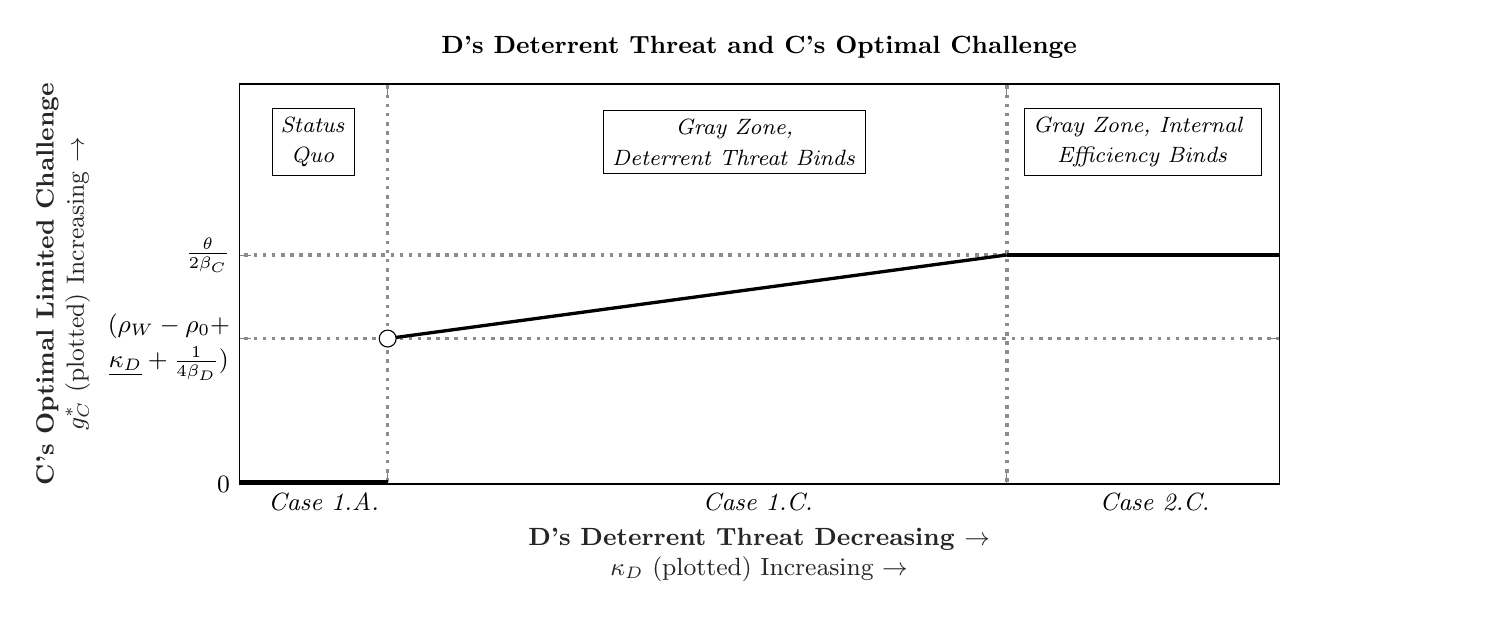
\begin{tikzpicture} 
    \small
    \begin{axis}[%
    width=5.2in,
    height=2in,
    at={(1.011in,0.642in)},
    scale only axis,
    xmin=0.01,
    xmax=0.22,
    xtick={0.01, 0.04,0.165,0.22},
    xticklabels={{},{\textit{Case 1.A.}$\,\,\,\,\,\,\,\,\,\,\,\,\,\,\,\,\,\,\,\,\,\,\,\,\,\,\,\,\,\,$},{\textit{Case 1.C.}$\;\;\;\;\;\;\;\;\;\;\;\;\;\;\;\;\;\;\;\;\;\;\;\;\;\;\;\;\;\;\;\;\;\;\;\;\;\;\;\;\;\;\;\;\;\;\;\;\;\;\;\;\;\;\;\;\;\;\;\;\;\;\;\;\;\;\;\;\;\;$},{\textit{Case 2.C.}$\;\;\;\;\;\;\;\;\;\;\;\;\;\;\;\;\;\;\;\;\;\;\;\;\;\;\;\;\;\;\;\;\;\;\;$}},
    xlabel style={font=\color{white!15!black},align=center},
    xlabel={\textbf{D's Deterrent Threat Decreasing $\rightarrow$} \\ $\kappa_D$ (plotted) Increasing $\rightarrow$ },
    ymin=0.7,
    ymax=1.25,
    ytick={0.7,.9, 1.0147},
    yticklabels={{0},{\shortstack{{}\\{}\\($\rho_{W}-\rho_{0}+$\\$\underline{\kappa_{D}}+\frac{1}{4\beta_{D}}$)}},{$\frac{\theta}{2\beta_C}$}},
    ylabel style={font=\color{white!15!black}, align=center},
    ylabel={\textbf{C's Optimal Limited Challenge} \\ $g_{C}^*$ (plotted) Increasing $\rightarrow$},
    axis background/.style={fill=white},
    title style={font=\bfseries},
    title={D's Deterrent Threat and C's Optimal Challenge},
    ]
    
    %
     
    \node[draw, align=center] at (0.025,1.17) {\footnotesize{\textit{Status}}\\ \footnotesize{\textit{Quo}}};
    
    
    \node[draw, align=center] at (0.11,1.17) {\footnotesize{\textit{Gray Zone,}} \\ \footnotesize{\textit{Deterrent Threat Binds}}}; 
    
    \node[draw, align=center] at (.1925,1.17) {\footnotesize{\textit{Gray Zone, Internal }} \\ \footnotesize{\textit{Efficiency Binds}}};
    
    %\node[draw, align=center] at (.1925,1.2) {\footnotesize{\textit{Gray Zone,}} \\ \footnotesize{\textit{Unconstrained}}}; 
    
    \addplot [color=white!55!black, dotted, line width=1.3pt, forget plot]
      table[row sep=crcr]{%
    0.04	0\\
    0.04	1.5\\
    };
    \addplot [color=white!55!black, dotted, line width=1.3pt, forget plot]
      table[row sep=crcr]{%
    0.165	0\\
    0.165	1.5\\
    };
    
    
    \addplot [color=white!55!black, dotted, line width=1.3pt, forget plot]
      table[row sep=crcr]{%
    0 	0.9\\
    .22	0.9\\
    };
    \addplot [color=white!55!black, dotted, line width=1.3pt, forget plot]
      table[row sep=crcr]{%
    0 	1.015\\
    .22	1.015\\
    };
    
    %Real lines
    
    \addplot [color=black, line width=1.2pt]
      table[row sep=crcr]{%
    0.01		0.703	\\
    0.04		0.703\\
    };
    
    
    \addplot [color=black, line width=1.2pt]
      table[row sep=crcr]{%
    0.04		0.9	\\
    0.165		1.015\\
    };
    
    
    \addplot [color=black, line width=1.2pt, forget plot]
      table[row sep=crcr]{%
    0.165	1.015	\\
    0.22		1.015	\\
    };
    
    
      
        \node at (0.04,0.207)  [circle,scale=0.7,minimum size=0.5pt,draw,fill=black!100] {};
        \node at (0.04,0.9)  [circle,scale=0.7,draw,fill=black!0] {};
    
    
      %          \node at (0.675,0.36) [circle,scale=0.7,minimum size=0.5pt,draw,fill=black!100] {};
       %         \node at (0.675,0.1) [circle,scale=0.7,draw,fill=black!0] {};
                
    
    
    \end{axis}
    \end{tikzpicture}
    \caption{Optimal Limited Challenge as D's Deterrent Threat Decreases}
    \floatnote{C's selected limited challenge intensity under a range of $\kappa_D$'s are plotted. We define $\underline{\kappa_{D}}$ implicitly as the value of D's war costs that satisfies $\theta=\frac{\beta_{C}\left(\rho_{W}-\rho_{0}+\underline{\kappa_{D}}+\frac{1}{4\beta_{D}}\right)^{2}}{\left(\rho_{W}-\rho_{0}+\underline{\kappa_{D}}-\frac{1}{4\beta_{D}}\right)}$. All equilibrium cases are described in Proposition 1. 
    %The x-axis endpoints are $\kappa_D=0.01$ and $\kappa_D=0.22$. 
    The parameters are $\rho_0=0.1$, $\rho_W=0.7$, $\beta_C=0.34$, $\kappa_{C}=0.5$, $\beta_D=1$, and $\theta=0.69$. To simplify labeling, y-axis not drawn to scale.}
    \label{fig:optimaldetdecrease}
    \end{figure}

Moving to the right---to Case 1.C. equilibrium space---because D is less willing to go to war, C can engage in enough limited challenges to make gray zone conflict worthwhile. Here the intensity of C's limited challenge is constrained by D's deterrent threat, so C can select more aggressive limited challenges as D's deterrent threat decreases.

In  Case 2.C, because D's deterrent threat has sufficiently declined, D is willing to tolerate aggressive limited challenges without escalating to war. Here, D's deterrent threat no longer binds, and instead C's limited challenge is constrained by C's internal efficiency constraint, which is not a function of D's deterrent threat.\footnote{The level of limited challenge that D would tolerate follows the trend of the diagonal line in the 1.C. region.}

Altogether, Figure \ref{fig:optimaldetdecrease} illustrates a natural intuition. As D's deterrent threat from war decreases, C can select more aggressive limited challenges without provoking D to war. This expands the possible set of limited challenges that will not trigger an escalation, thus resulting in a greater intensity of gray zone conflict, until C's internal efficiency constraint binds and C no longer finds more gray zone conflict worthwhile.

\subsection{On the Challenger's Resolve and Conflict Intensity}
As the challenger becomes more resolved or cares more about the policy issue ($\theta$ increases), the challenger's chosen level of limited challenge ($g_{C}^{*}$) weakly increases, unless its resolve is so high that it forgoes gray zone conflict and resorts to war. For example, during the Syrian Civil War, while both Moscow and the Syrian Ba'athist party clearly preferred retaining Bashar al-Assad's power, the Ba'athist party was presumably more resolved and fought harder than Russia.
%than officials in Moscow. Thus, Ba'athist troops were fully committed to the civil war, while Russian forces engaged in much more limited operations. 
Consider a setting where 
%the defender has a weak deterrent threat and 
the challenger optimally pursues a limited challenge to the status quo based on its own internal balancing of costs and benefits (the challenger's internal efficiency constraint binds). As the challenger's resolve increases, the challenger benefits more from shifting the status quo and is willing to select more aggressive limited challenges. However, a sufficiently highly resolved challenger could be willing to select a limited challenge intensity that exceeds the defender's tolerance within gray zone conflict. For these high levels of resolve, the challenger must either choose a non-internally-optimal intensity of its limited challenges to keep the defender from going to war---reflecting the external constraint of the defender's deterrent threat---or accept escalation to war.

\textbf{\textit{Observation 2:}}\textit{ As the challenger's resolve increases, the challenger selects weakly more intense limited challenges, or may forgo gray zone conflict for war.}

Observation 2 follows naturally from Proposition 1, and Figure \ref{fig:optimalresolveincrease} illustrates one example of Observation 2. Moving from left-to-right, C's resolve $\theta$ is increasing. For the lowest resolve considered---the region where the equilibrium is described in Case 2.A.---C is not particularly resolved, and does not stand to gain sufficiently by altering the status quo. Because of this, C makes do with the status quo.

    \begin{figure}[h]
    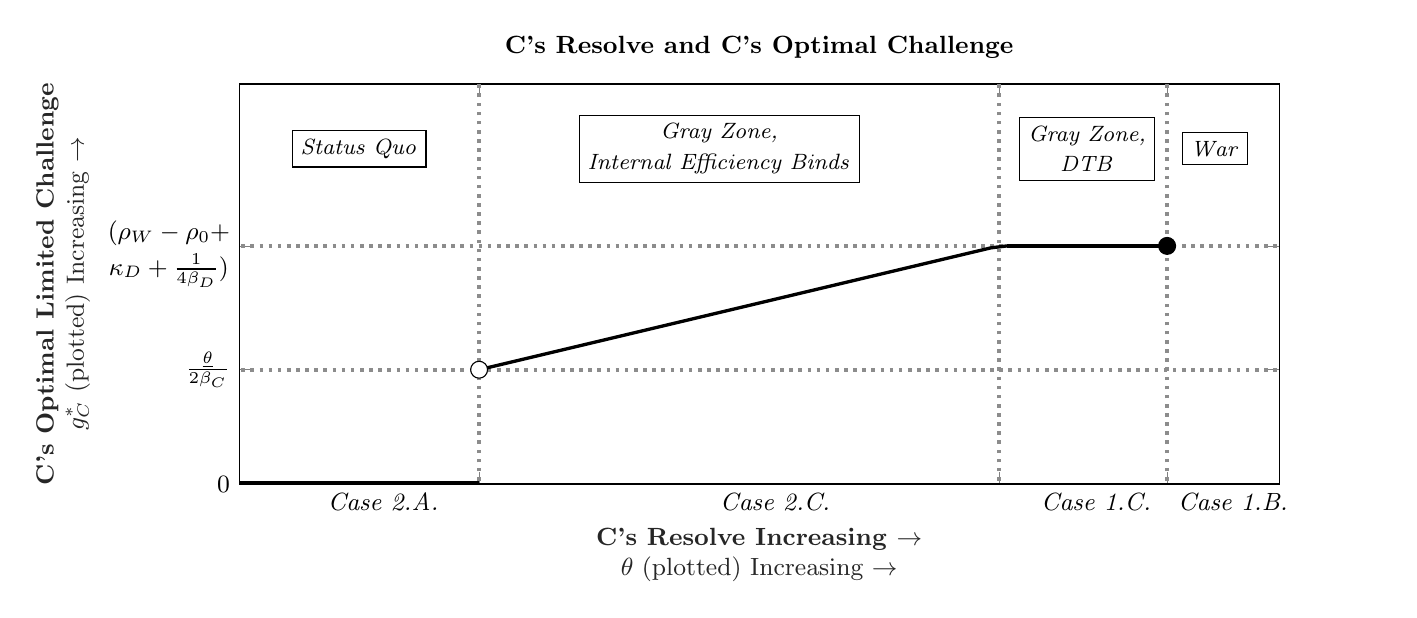
\begin{tikzpicture} 
    \small
    \begin{axis}[%
    width=5.2in,
    height=2in,
    at={(1.011in,0.642in)},
    scale only axis,
    xmin=1.27,
    xmax=1.4,
    xtick={1.3,1.365,1.386,1.4},
    xticklabels={{\textit{Case 2.A.$\;\;\;\;\;\;\;\;\;\;\;\;\;\;\;\;\;\;\;\;\;\;\;\;\;\;\;$}},{\textit{Case 2.C.$\;\;\;\;\;\;\;\;\;\;\;\;\;\;\;\;\;\;\;\;\;\;\;\;\;\;\;\;\;\;\;\;\;\;\;\;\;\;\;\;\;\;\;\;\;\;\;\;\;\;\;\;\;\;\;\;\;\;\;\;\;\;\;$}},{\textit{Case 1.C.}$\;\;\;\;\;\;\;\;\;\;\;\;\;\;\;\;\;\;\;\;$},{\textit{Case 1.B.}$\;\;\;\;\;\;\;\;\;\;\;\;\;$}},
    xlabel style={font=\color{white!15!black},align=center},
    xlabel={\textbf{C's Resolve Increasing $\rightarrow$} \\ $\theta$ (plotted) Increasing $\rightarrow$},
    ymin=0.62,
    ymax=.725,
    ytick={0.62,0.65, 0.6825},
    yticklabels={{0},{$\frac{\underline{\theta}}{2\beta_{C}}$},{\shortstack{{}\\{}\\($\rho_{W}-\rho_{0}+$\\$\kappa_{D}+\frac{1}{4\beta_D}$)}}},
    ylabel style={font=\color{white!15!black}, align=center},
    ylabel={\textbf{C's Optimal Limited Challenge} \\ $g_{C}^*$ (plotted) Increasing $\rightarrow$},
    axis background/.style={fill=white},
    title style={font=\bfseries},
    title={C's Resolve and C's Optimal Challenge},
    ]
    
    %
     
    \node[draw, align=center] at (1.285,0.708) {\footnotesize{\textit{Status Quo}}};
    \node[draw, align=center] at (1.33,0.708) {\footnotesize{\textit{Gray Zone,}} \\ \footnotesize{\textit{Internal Efficiency Binds}}}; 
    \node[draw, align=center] at (1.376,0.708) {\footnotesize{\textit{Gray Zone,}} \\ \footnotesize{\textit{DTB}}}; 
    \node[draw, align=center] at (1.392,0.708) {\footnotesize{\textit{War}}};
    
    %\node[draw, align=center] at (.1925,1.2) {\footnotesize{\textit{Gray Zone,}} \\ \footnotesize{\textit{Unconstrained}}}; 
    
    %BEGIN DOTTED LINES
    \addplot [color=white!55!black, dotted, line width=1.3pt, forget plot]
      table[row sep=crcr]{%
    1.3	0\\
    1.3	1\\
    };
    \addplot [color=white!55!black, dotted, line width=1.3pt, forget plot]
      table[row sep=crcr]{%
    1.365	0\\
    1.365	1\\
    };
    
    \addplot [color=white!55!black, dotted, line width=1.3pt, forget plot]
      table[row sep=crcr]{%
    1.386 	0\\
    1.386	0.9\\
    };
    \addplot [color=white!55!black, dotted, line width=1.3pt, forget plot]
      table[row sep=crcr]{%
    1.26 	0.65\\
    1.4	0.65\\
    };
    
    \addplot [color=white!55!black, dotted, line width=1.3pt, forget plot]
      table[row sep=crcr]{%
    1.26 	0.6825\\
    1.4	0.6825\\
    };
    %%END DOTTED LINES
    
    \addplot [color=black, line width=1.2pt]
      table[row sep=crcr]{%
    1.27		0.6204	\\
    1.3			0.6204\\
    };
    
    
    \addplot [color=black, line width=1.2pt]
      table[row sep=crcr]{%
    1.300	0.65	\\
    1.302	0.651	\\
    1.304	0.652	\\
    1.306	0.653	\\
    1.308	0.654	\\
    1.31	0.655	\\
    1.312	0.656	\\
    1.314	0.657	\\
    1.316	0.658	\\
    1.318	0.659	\\
    1.32	0.66	\\
    1.322	0.661	\\
    1.324	0.662	\\
    1.326	0.663	\\
    1.328	0.664	\\
    1.33	0.665	\\
    1.332	0.666	\\
    1.334	0.667	\\
    1.336	0.668	\\
    1.338	0.669	\\
    1.34	0.67	\\
    1.342	0.671	\\
    1.344	0.672	\\
    1.346	0.673	\\
    1.348	0.674	\\
    1.35	0.675	\\
    1.352	0.676	\\
    1.354	0.677	\\
    1.356	0.678	\\
    1.358	0.679	\\
    1.36	0.68	\\
    1.362	0.681	\\
    1.364	0.682	\\
    1.366	0.6825	\\
    };
    
    
    \addplot [color=black, line width=1.2pt, forget plot]
      table[row sep=crcr]{%
    1.366	0.6825	\\
    1.386		0.6825	\\
    };
    
    \addplot [color=black, line width=1.2pt, forget plot]
      table[row sep=crcr]{%
    1.386	0.5003	\\
    1.4		0.5003	\\
    };
    
    
    
      
       \node at (1.3,0.502)  [circle,scale=0.7,minimum size=0.5pt,draw,fill=black!100] {};
        \node at (1.3,0.65)  [circle,scale=0.7,draw,fill=black!0] {};
    
       \node at (1.386,0.6825)  [circle,scale=0.7,minimum size=0.5pt,draw,fill=black!100] {};
        \node at (1.386,0.502)  [circle,scale=0.7,draw,fill=black!0] {}; 
    
      %          \node at (0.675,0.36) [circle,scale=0.7,minimum size=0.5pt,draw,fill=black!100] {};
       %         \node at (0.675,0.1) [circle,scale=0.7,draw,fill=black!0] {};
                
    
    
    \end{axis}
    \end{tikzpicture}
    \caption{Optimal limited challenge as C's Resolve Increases}
    \floatnote{C's selected limited challenge intensity under a range of $\theta$'s are plotted. We define $\underline{\theta}=\frac{2\beta_{C}}{\beta_{D}}$. ``DTB'' is an abbreviation for ``Deterrent Threat Binds.'' All equilibrium cases are described in Proposition 1. 
    %The x-axis endpoints are $\theta=$ and $\theta=1.4$. 
    The parameters are $\rho_0=0$, $\rho_W=0.42$, $\beta_C=1$, $\kappa_{C}=0.5525$, $\beta_D=1.53$, and $\kappa_D=0.1$. To simplify labeling, y-axis not drawn to scale. We illustrate C selecting $w_{A}^{*}=1$ as C selecting $g_{C}^{*}=0.$}
    \label{fig:optimalresolveincrease}
    \end{figure}

In Case 2.C, because C is more resolved to alter the status quo, C does best by engaging in limited challenges (gray zone). Here C's internal efficiency constraint binds, meaning C's selected limited challenge is increasing in C's resolve.

In Case 1.C, here C's resolve is even higher, but D's deterrent threat binds. C is resolved enough to engage in aggressive limited challenges beyond what D would tolerate (a level that would provoke D to escalate to war),\footnote{C's nominal willingness to challenge grows along the trend line from the Case 2.C.} but C is not resolved enough to go to war. As a result, C selects a level of limited challenge bound by D's indifference threshold between war and gray zone conflict, which is unchanging in C's resolve.

Finally, in Case 1.B, C's resolve has increased to the point where the level of limited challenges within gray zone conflict tolerated by D is not productive enough for C. Thus, in this region, C optimally goes to war over the issue.

\subsection{On the Challenger's Gray Zone Costs and Conflict Intensity}
As the challenger's costs from gray zone conflict decrease ($\beta_{C}$ decreases), the challenger will select weakly more aggressive limited challenges ($g_{C}^{*}$). When the internal efficiency constraint binds, the challenger's selection of their limited challenges will increase as their costs decrease. When the external deterrent threat binds, the challenger's selection of their limited challenge does not vary with their costs, but rather is dictated by the defender's willingness to go to war, which is static.

\textbf{\textit{Observation 3:}}\textit{ As C's gray zone costs decrease, C selects weakly more intense limited challenges, and may forgo accepting the status quo or war for gray zone conflict.}
 
Figure \ref{fig:optimalcostvary} illustrates one example of Observation 3. Given the self-evident nature of this finding,
%(C wanting to do more of something when it is cheaper to do so), 
we do not discuss these conditions at length.

    \begin{figure}[h]
    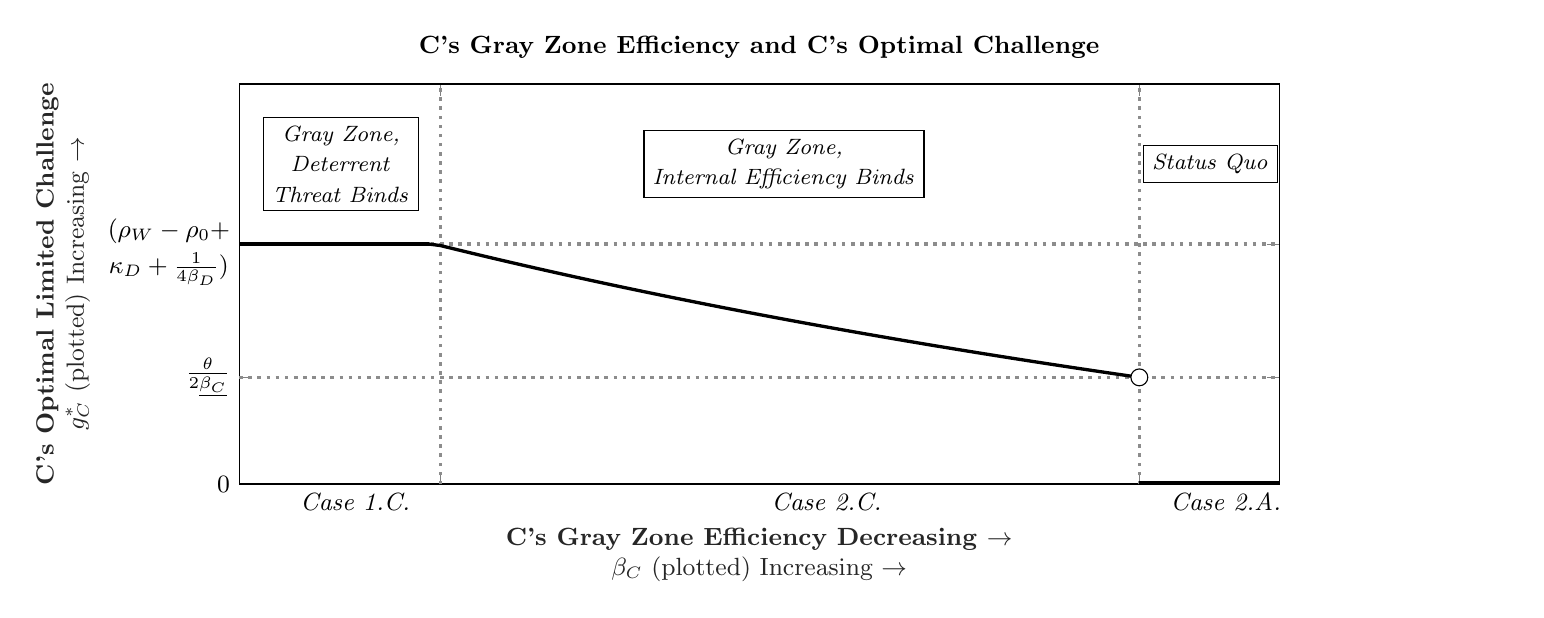
\begin{tikzpicture} 
    \small
    \begin{axis}[%
    width=5.2in,
    height=2in,
    at={(1.011in,0.642in)},
    scale only axis,
    xmin=0.087,
    xmax=.1309,
    xtick={0.087, 0.0955,0.125,0.1309},
    xticklabels={{},{\textit{Case 1.C.}$\;\;\;\;\;\;\;\;\;\;\;\;\;\;\;\;\;\;\;\;\;\;\;\;$},{\textit{Case 2.C.}$\;\;\;\;\;\;\;\;\;\;\;\;\;\;\;\;\;\;\;\;\;\;\;\;\;\;\;\;\;\;\;\;\;\;\;\;\;\;\;\;\;\;\;\;\;\;\;\;\;\;\;\;\;\;\;\;\;\;\;\;\;\;\;\;\;\;\;\;\;\;\;\;\;\;\;\;\;\;\;\;\;\;\;\;\;\;\;\;$},{\textit{Case 2.A.}$\;\;\;\;\;\;\;\;\;\;\;\;\;\;\;$}},
    xlabel style={font=\color{white!15!black},align=center},
    xlabel={\textbf{C's Gray Zone Efficiency Decreasing $\rightarrow$} \\ $\beta_C$ (plotted) Increasing $\rightarrow$ },
    ymin=0.6,
    ymax=1.35,
    ytick={0.6, 0.8, 1.05,1.35},
    yticklabels={{0},{$\frac{\theta}{2\underline{\beta_C}}$},{\shortstack{{}\\{}\\($\rho_{W}-\rho_{0}+$\\$\kappa_{D}+\frac{1}{4\beta_D}$)}}},
    ylabel style={font=\color{white!15!black}, align=center},
    ylabel={\textbf{C's Optimal Limited Challenge} \\ $g_{C}^*$ (plotted) Increasing $\rightarrow$},
    axis background/.style={fill=white},
    title style={font=\bfseries},
    title={C's Gray Zone Efficiency and C's Optimal Challenge},
    ]
    
    %
     
    
    
    
    \addplot [color=white!55!black, dotted, line width=1.3pt, forget plot]
      table[row sep=crcr]{%
    0.087 	0.8\\
    0.1309	0.8\\
    };
    \addplot [color=white!55!black, dotted, line width=1.3pt, forget plot]
      table[row sep=crcr]{%
    .087	1.05\\
    0.1309	1.05\\
    };
    
    \node[draw, align=center] at (0.128,1.2) {\footnotesize{\textit{Status Quo}}};
    
    \node[draw, align=center] at (0.11,1.2) {\footnotesize{\textit{Gray Zone,}}\\ \footnotesize{\textit{Internal Efficiency Binds}}}; 
    
    \node[draw, align=center] at (.0913,1.2) {\footnotesize{\textit{Gray Zone,}} \\ \footnotesize{\textit{Deterrent}}\\ \footnotesize{\textit{Threat Binds}}};
    
    %OLD
    %\node[draw, align=center] at (.1925,1.2) {\footnotesize{\textit{Gray Zone,}} \\ \footnotesize{\textit{Unconstrained}}}; 
    
    \addplot [color=white!55!black, dotted, line width=1.3pt, forget plot]
      table[row sep=crcr]{%
    0.0955	0\\
    0.0955	1.5\\
    };
    \addplot [color=white!55!black, dotted, line width=1.3pt, forget plot]
      table[row sep=crcr]{%
    0.125	0\\
    0.125	1.5\\
    };
    
    
    
    \addplot [color=black, line width=1.2pt]
      table[row sep=crcr]{%
    0.087	1.05	\\
    0.0915	1.05	\\
    0.092	1.05	\\
    0.0925	1.05	\\
    0.093	1.05	\\
    0.0935	1.05	\\
    0.094	1.05	\\
    0.095	1.05	\\
    };
    
    
    \addplot [color=black, line width=1.2pt]
      table[row sep=crcr]{%
    0.095	1.05	\\
    0.0955	1.047120419	\\
    0.096	1.041666667	\\
    0.0965	1.03626943	\\
    0.097	1.030927835	\\
    0.0975	1.025641026	\\
    0.098	1.020408163	\\
    0.0985	1.015228426	\\
    0.099	1.01010101	\\
    0.0995	1.005025126	\\
    0.1	1	\\
    0.1005	0.995024876	\\
    0.101	0.99009901	\\
    0.1015	0.985221675	\\
    0.102	0.980392157	\\
    0.1025	0.975609756	\\
    0.103	0.970873786	\\
    0.1035	0.966183575	\\
    0.104	0.961538462	\\
    0.1045	0.956937799	\\
    0.105	0.952380952	\\
    0.1055	0.947867299	\\
    0.106	0.943396226	\\
    0.1065	0.938967136	\\
    0.107	0.934579439	\\
    0.1075	0.930232558	\\
    0.108	0.925925926	\\
    0.1085	0.921658986	\\
    0.109	0.917431193	\\
    0.1095	0.913242009	\\
    0.11	0.909090909	\\
    0.1105	0.904977376	\\
    0.111	0.900900901	\\
    0.1115	0.896860987	\\
    0.112	0.892857143	\\
    0.1125	0.888888889	\\
    0.113	0.884955752	\\
    0.1135	0.881057269	\\
    0.114	0.877192982	\\
    0.1145	0.873362445	\\
    0.115	0.869565217	\\
    0.1155	0.865800866	\\
    0.116	0.862068966	\\
    0.1165	0.858369099	\\
    0.117	0.854700855	\\
    0.1175	0.85106383	\\
    0.118	0.847457627	\\
    0.1185	0.843881857	\\
    0.119	0.840336134	\\
    0.1195	0.836820084	\\
    0.12	0.833333333	\\
    0.1205	0.829875519	\\
    0.121	0.826446281	\\
    0.1215	0.823045267	\\
    0.122	0.819672131	\\
    0.1225	0.816326531	\\
    0.123	0.81300813	\\
    0.1235	0.809716599	\\
    0.124	0.806451613	\\
    0.125	0.80\\
    };
    
    
    \addplot [color=black, line width=1.2pt, forget plot]
      table[row sep=crcr]{%
    0.125	0.603	\\
    0.1309	0.603	\\
    };
    
      
        \node at (.125,0.207)  [circle,scale=0.7,minimum size=0.5pt,draw,fill=black!100] {};
        \node at (0.125,0.8)  [circle,scale=0.7,draw,fill=black!0] {};
    
    
      %          \node at (0.675,0.36) [circle,scale=0.7,minimum size=0.5pt,draw,fill=black!100] {};
       %         \node at (0.675,0.1) [circle,scale=0.7,draw,fill=black!0] {};
                
    
    
    \end{axis}
    \end{tikzpicture}
    \caption{Optimal limited challenge as C's costs of limited challenges vary}
    \floatnote{C's selected limited challenge intensity under a range of $\beta_C$'s are plotted. We define $\underline{\beta_C}$ as $\frac{\theta}{2\underline{\beta_{C}}}=\rho_{W}-\rho_{0}+\kappa_{D}+\frac{1}{4\beta_{D}}$. All equilibrium cases are described in Proposition 1. 
    %The x-axis endpoints are $\beta_C=0.087$ and $\beta_C=0.1309$.
    The parameters are are $\rho_0=0.1$, $\rho_W=0.8$, $\kappa_D=0.15$, $\kappa_{C}=0.2$, $\beta_D=1.25$, and $\theta=0.2$. To simplify labeling, y-axis not drawn to scale..}
    \label{fig:optimalcostvary}
    \end{figure}

\section{Empirical Application: Russian Efforts in the Gray Zone}
We empirically assess our argument by analyzing data on the scope and intensity of Russian foreign interventions over the past two decades. Quantitative analysis supports the hypothesis discussed in Observation 1: that Russia chooses its level of provocation in response to NATO's implicit deterrent threat in a given location. A secondary hypothesis allows us to operationalize the primary one: we expect the credibility of NATO deterrence to vary inversely with the military loss of strength gradient \citep{boulding_conflictdefensegeneral_1962}. Geography is not the focus of this article, but we use it as an instrument to map variation in the credibility of deterrence. We thus expect Russian military actions to appear more vigorous as the constraints of deterrence are relaxed.

We focus on Russia because its interventions are extensively referenced as paradigmatic examples of gray zone conflict \citep{marten_putinchoicesexplaining_2015, driscoll_friendsthesebrinkmanship_2016, chivvis_hybridwarrussian_2017}. From 1994 to 2018, Russia has been involved in election interference in the United Kingdom and Moldova, cyberattacks in Estonia and Georgia, and special operations in Ukraine and elsewhere. Russia's military adventures are the ``most likely'' cases for the argument that gray zone conflict is an effective and low-cost innovation for revising the status quo. The diversity of Russian targets and means employed provides an opportunity to conduct a controlled comparison of Russian choices under different deterrent circumstances. We present a simple, large-N statistical analysis where we test the implications of the model on Russian decision making while controlling for a number of relevant factors. By no means is this analysis causal, as our key independent variables---NATO membership, for example---are certainly not an exogenous treatment. Our results should be viewed as suggestive and should be taken with the necessary caveats. We then undertake a closer qualitative analysis of three cases: Estonia, Ukraine, and Georgia. We find that the possibility of a NATO intervention is associated with more limited gray zone operations, suggesting that NATO's deterrent threat shapes Russian gray zone behavior.

\subsection{Data}
Admittedly, data on Russian gray zone interventions are themselves a bit ambiguous. Most quantitative studies of gray zone operations focus on a particular type of gray zone activity, like cyber in the case of the Dyadic Cyber Incident and Dispute (DCID) data or electoral interference in the case of the Russian Electoral Interventions (REI) data \citep{valeriano_dynamicscyberconflict_2014, casey_russianelectoralinterventions_2017}. Consequently, they cover almost entirely distinct samples with significant differences concerning the severity of Russian attacks.\footnote{Indeed, the only country-year that appears in both datasets is Ukraine 2014.}

To address these deficiencies and discrepancies, we construct a new, expanded dataset including 82 cases of Russian intervention from 1994 to 2018. DCID and REI together describe 71 unique cases of Russian aggression that have either included some degree of cyber intervention or were cases of electoral interference. We identify 10 additional instances of Russian cyberattacks in the coding period that are not listed in previous datasets. Most of these new cases involve cyber conflict after 2011 (the latest year in DCID) that were non-electoral (the universe of cases in REI). We also include 3 cases of non-cyber Russian action from the International Crisis Behavior (ICB) dataset \citep{singer_capabilitydistributionuncertainty_1972}. For each incident, we create a new coding of the intensity of Russian attacks by coding whether Russia used five different types of military force in ascending order of intensity: (1) information operations (social media and disinformation), (2) cyber operations that result in disruption of infrastructure (service denial or industrial control system attacks), (3) overt use of special operations or unattributed military forces, (4) conventional air or sea forces, and (5) conventional ground forces.\footnote{We include conventional military interventions that occur alongside gray zone operations so as to avoid selecting on the dependent variable \citep{healey_escalationinversionother_2020, mares_georgia2008conflict_2020}.} This data is then aggregated to the country-year level with a coding for the highest level of intensity of Russian intervention against each country in each year. Our dependent variable is thus an ordinal variable coded 5 for the highest level of intensity down to 0 for country-years experiencing no Russian attack.

Figure \ref{fig:intensity} plots the count and average intensity of Russian gray zone operations since 1994. Contrary to descriptions of gray zone conflict as a new means of non-deterrable aggression or the product of an expansive technological portfolio, there does not appear to be a clear temporal pattern in the intensity or frequency of activity. Instead, 2004 represents the most intense overall Russian interventions and 2014 experienced the highest number of interventions (most of which were associated with Ukraine).

    \begin{figure}[H]
		\centering
		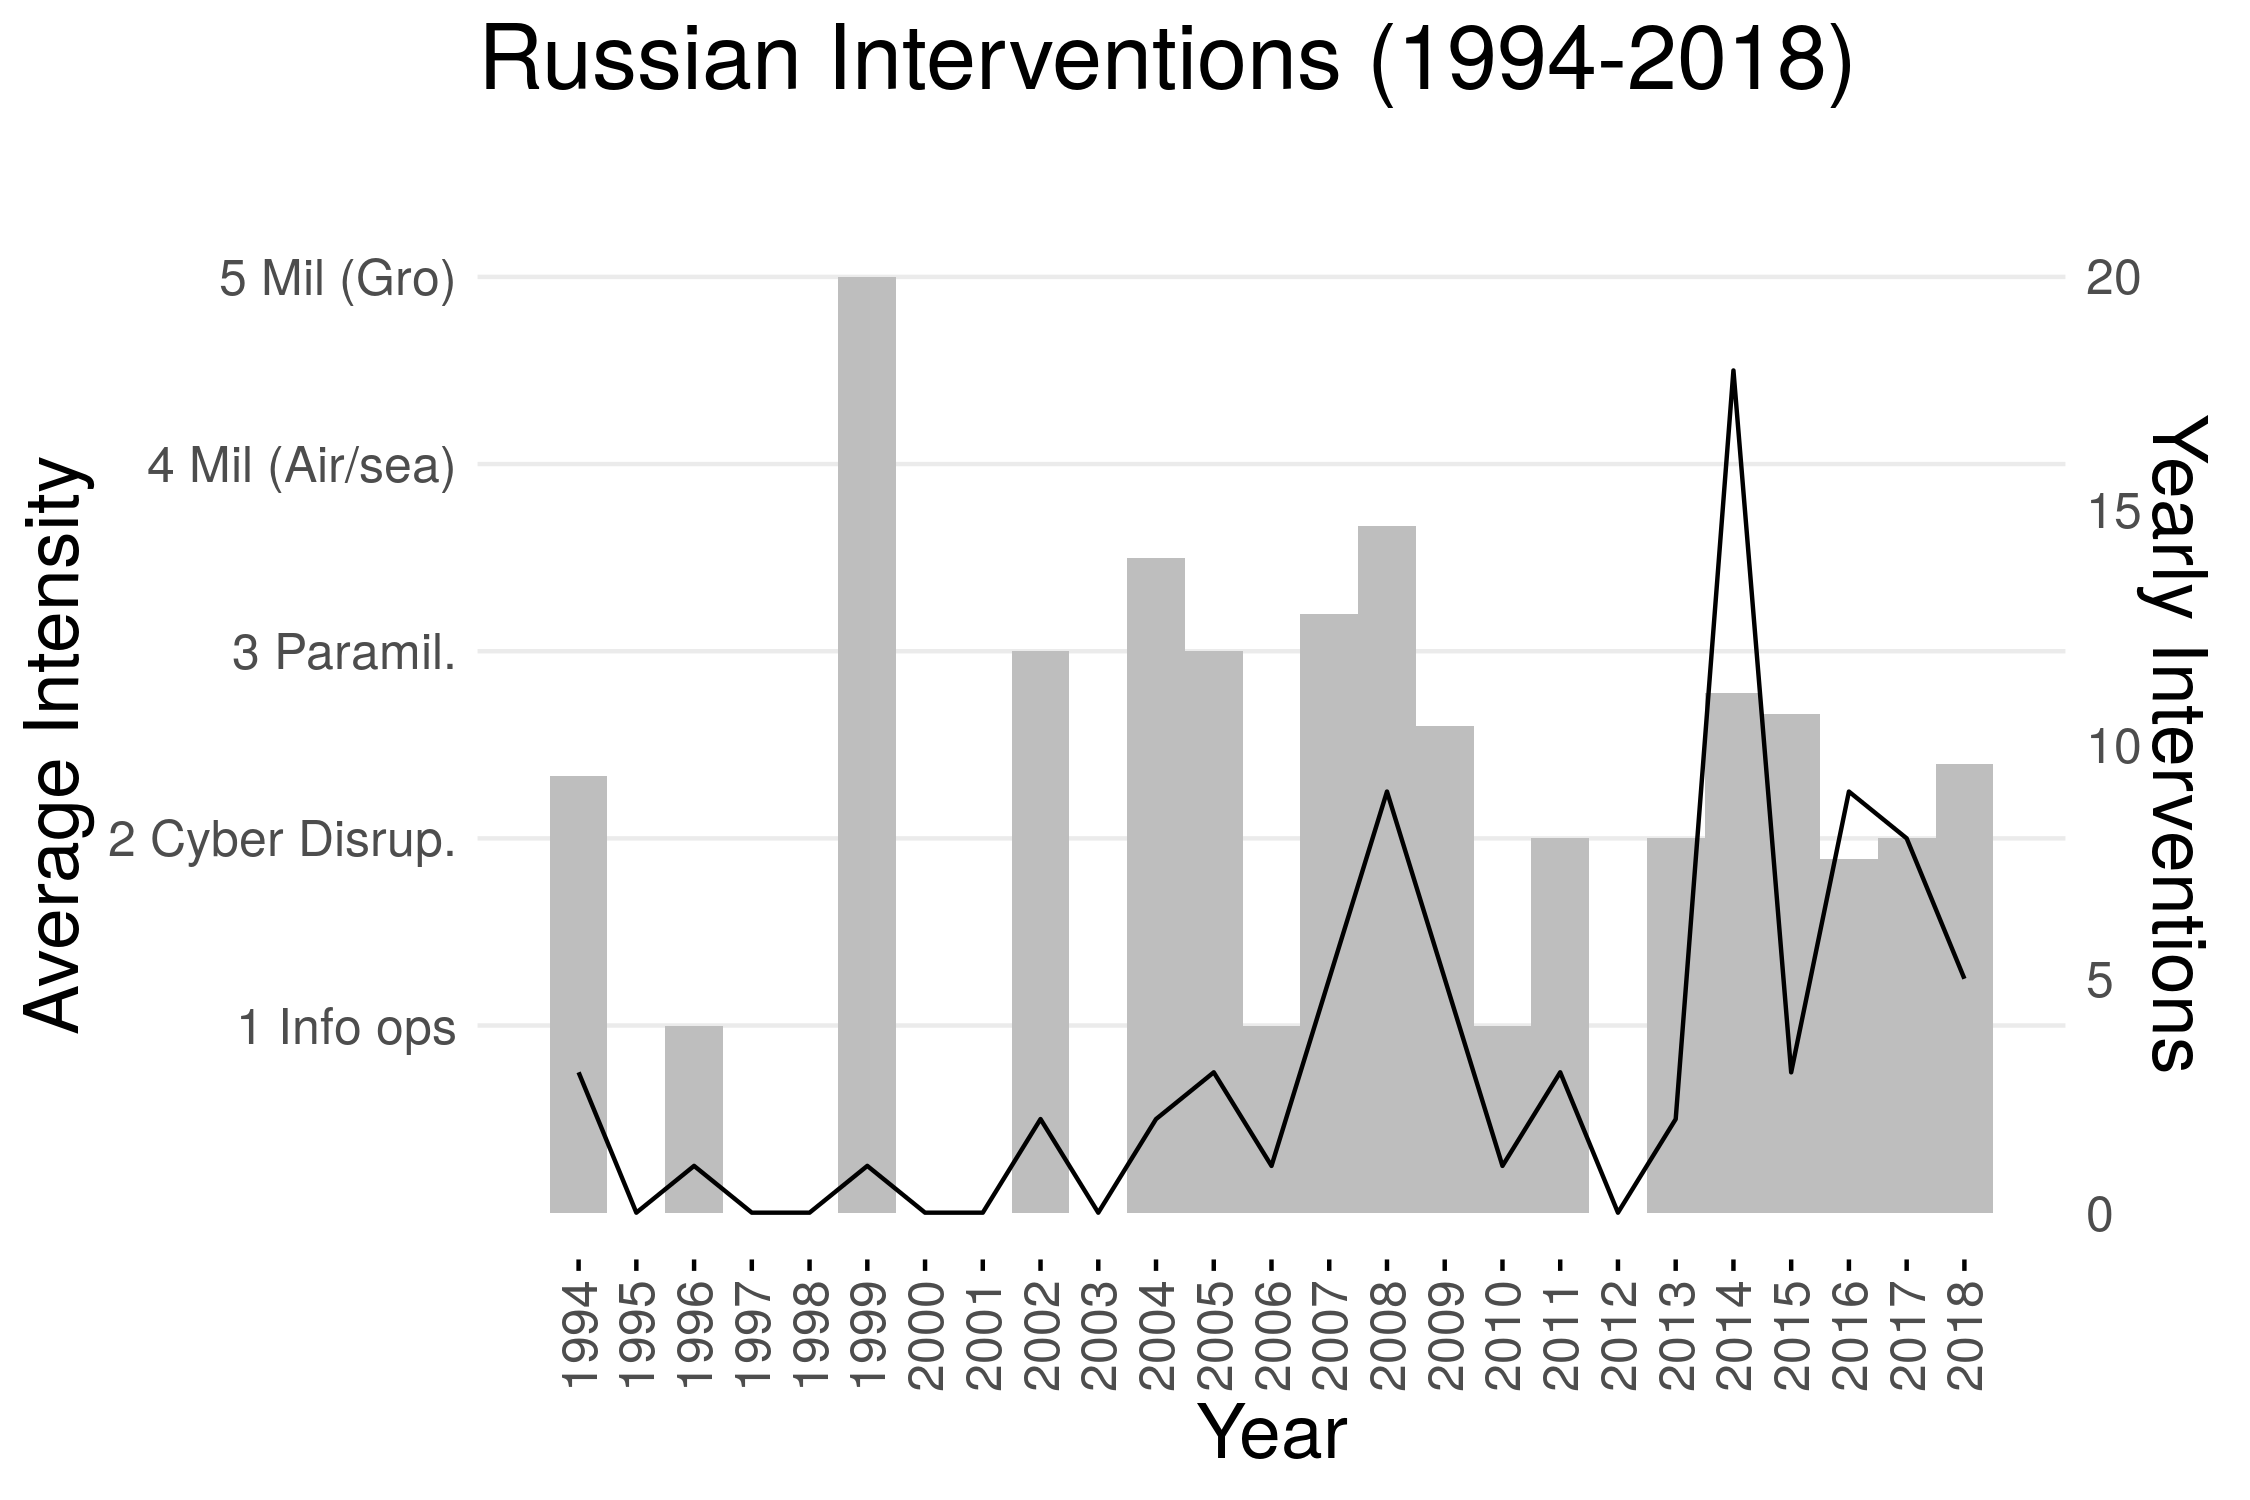
\includegraphics[width = \textwidth]{average_intensity_russian_aggression.png}
		\caption{Intensity of Russian intervention across time}
		\floatnote{The line represents the annual average of intensity. Bars denote the number of interventions per year.}
    \label{fig:intensity}
    \end{figure}

Figure \ref{fig:map} depicts a pattern of the geographical coverage of Russian conflict events in Europe. Russia appears to be willing to use more force in countries in its ``near abroad,'' relative to countries further away. Interpreting this geographic pattern on its own is difficult, as distance from Russia is plausibly related to Russian interest or resolve, Russia's ease of conducting operations, or the impact, or even the determinants of NATO membership. This pattern thus  highlights the need for a more sophisticated statistical analysis.

	\begin{figure}[H]
		\centering
		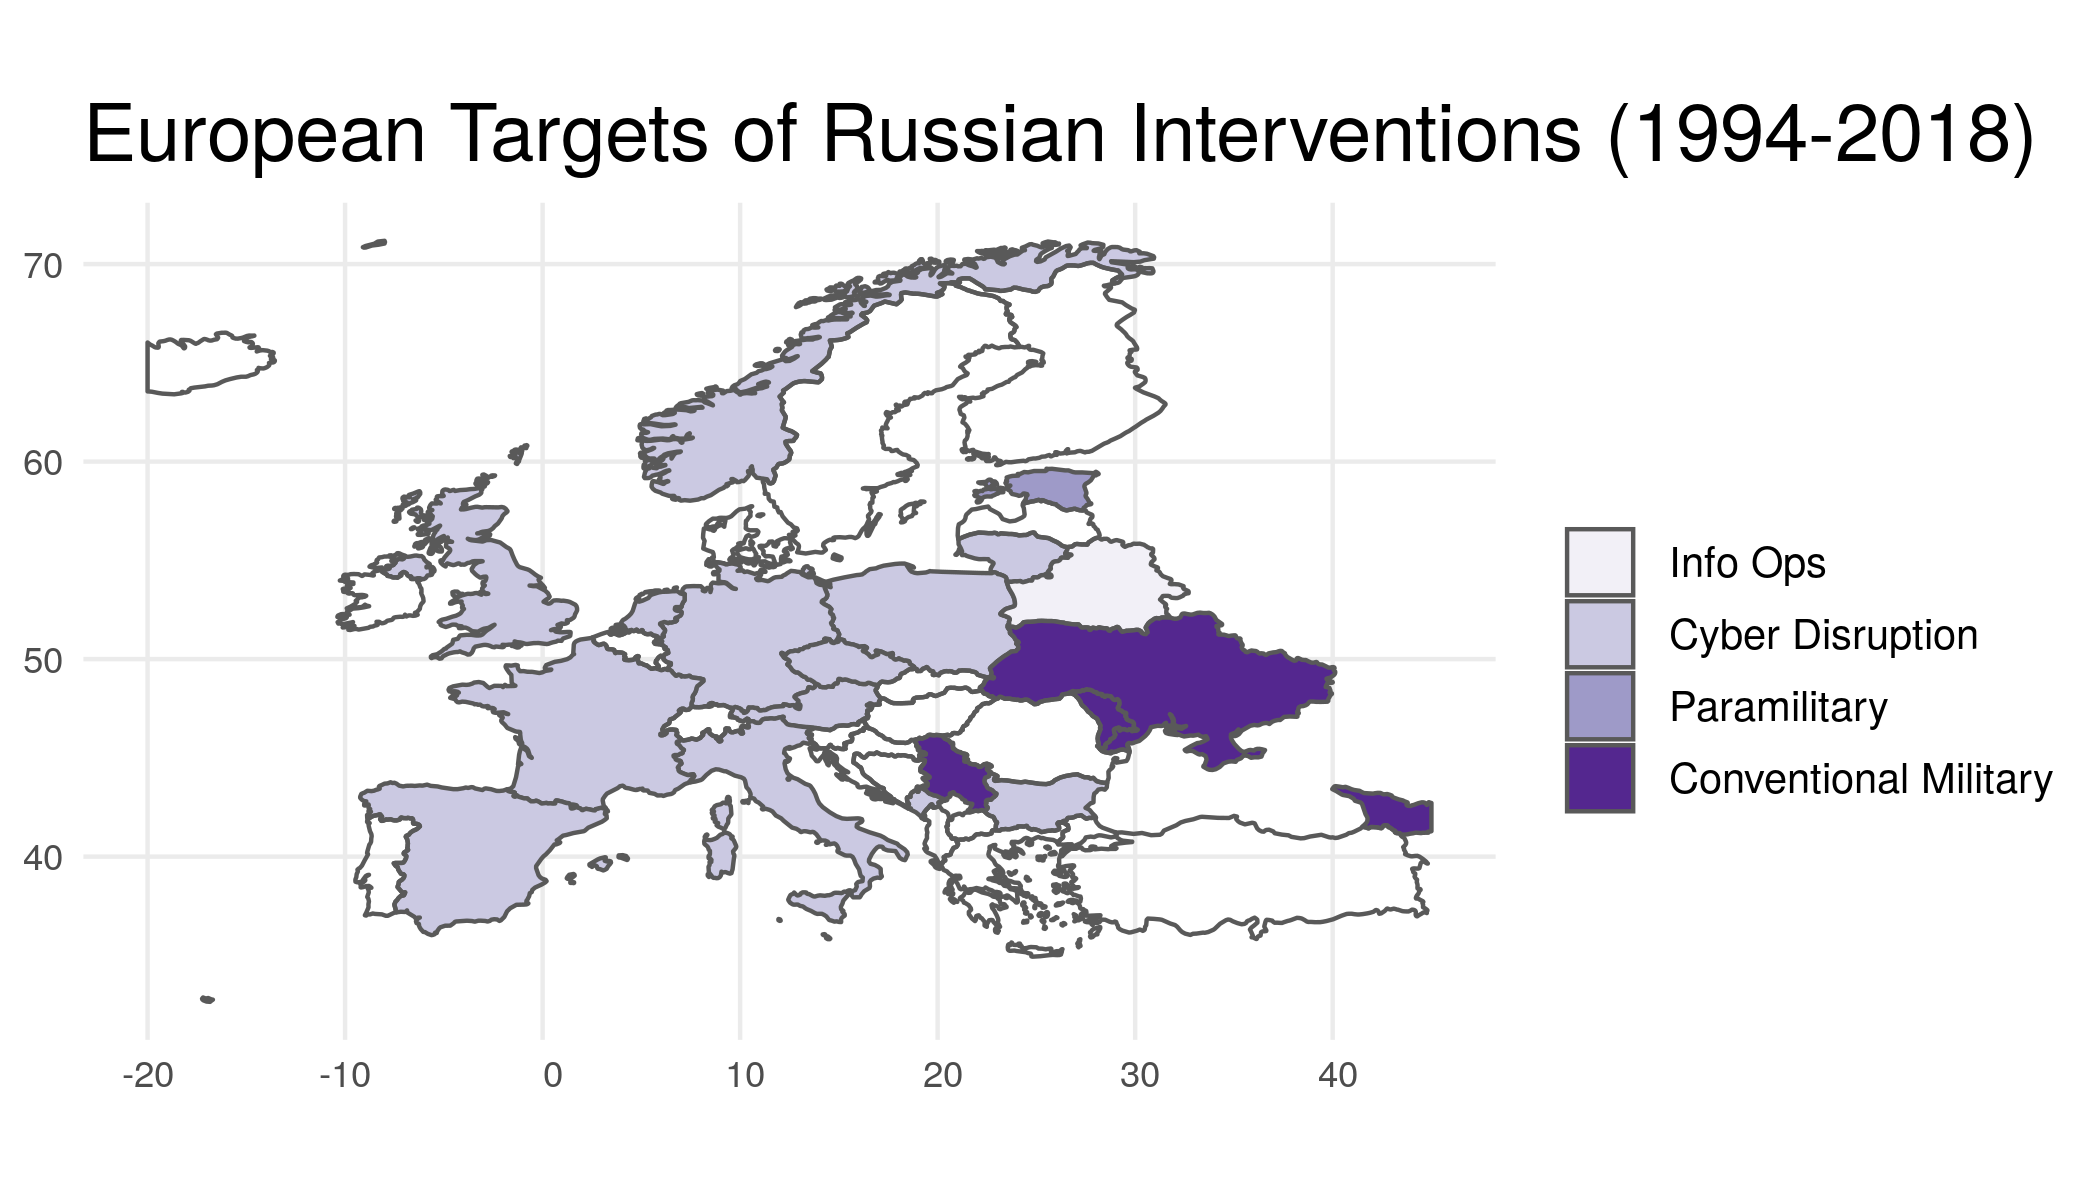
\includegraphics[width = \textwidth]{map_aggregate_europe.png}
		\caption{Geographic representation of Russia intervention}
		\floatnote{Shading represents the highest intensity of Russian intervention in each European state.}
		\label{fig:map}
	\end{figure}

Now we discuss our independent variables. Consistent with the discussion on the external deterrent threat (Observation 1), we propose that the external deterrent threat from war is a key driver of Russian gray zone behavior. We operationalize this concept through a dummy variable for NATO membership. NATO members plausibly possess lower costs for fighting---since they can rely on collective security. They may thus have a reduced willingness to tolerate aggressive low-level behavior from Russia. If Russia is responding to NATO's deterrent threat, we expect NATO states to experience less intense Russian activity. 

Consistent with the discussion of the internal-efficiency constraint (Observations 2 and 3), insofar as military power is affected by a loss of strength gradient \citep{corbett_principlesmaritimestrategy_1911, posen_commandcommonsmilitary_2003}, we propose the intensity of Russian gray zone operations could decrease as Russia has less resolve over the issue, or faces greater costs for conducting operations.\footnote{We only analyze this variable in models that also include a NATO membership covariate.} We operationalize Russian resolve and gray zone efficacy jointly through a variable of the logged minimum distance between Russia and each potential-target state, as we expect Russia to care more about states on its periphery and to more easily conduct operations in its proximity.

We also include a series of control variables. We include a democracy dummy for states with a Polity V score greater or equal to 6 to control for potential Russian eagerness to target democracies \citep{early_nuclearweaponsexistential_2018}. A state's possession of nuclear weapons may also alter Russia's calculus about how to pursue aggressive actions, so we include a dummy variable identifying whether a country-year is a nuclear state \citep{gartzke_strategicapproachnuclear_2009}. We include GDP per capita and the log of population as larger, richer states could afford more opportunities for Russian interventions, especially cyber interventions \citep{beckley_economicdevelopmentmilitary_2010}. Finally, we include military expenditure data from SIPRI since it influences both alliance decisions and the cost of undertaking aggression against an adversary \citep{omitoogun_militaryexpendituredata_2006}. Summary statistics for all variables are included in the Online Appendix.

\subsection{Model and Results}
Because our outcome is an ordinal value, we estimate a series of ordered probit models with year fixed-effects and standard errors clustered by country. Our unit of analysis is the country-year. We run three empirical models on two samples. On the models, first we estimate the relationship between the intensity of Russian intervention and NATO membership and minimum distance from Russia without any control variables. Second, we re-run the first model  while also controlling for the range of variables indicated above. We exclude military spending from the second model because it is missing across the entire panel for countries like Yugoslavia and Bosnia \& Herzegovina. In model 3, we include the military spending variable. We operationalize military power using population and SIPRI data on military expenditure. On the samples, our first sample (models (1)-(3)) includes all European states. We define state membership using the Gleditsch and Ward state list and continent location using the World Bank Development Indicator \citep{gleditsch_revisedlistindependent_1999}. This excludes micro-states with less than 250,000 people like Liechtenstein and San Marino. The downside is this sample may include states that are not of interest to Russia and may fall outside the scope of our model (for example, Luxembourg). To address this, our second sample (models (4)-(6)) represents "relevant European states," includes only European states that meet any of the three criteria: a) targets of a Russian attack from 1945-1993 as identified in the Militarized Interstate Dispute (MID) or International Crisis Behavior (ICB) datasets, b) Former Soviet Union or Warsaw Pact states, or c) states that are contiguous with Russia.


\begin{table}[h]
\begin{center}
\begin{tabular}{l c c c c c c}
\hline
 & \multicolumn{3}{c}{Full sample} & \multicolumn{3}{c}{Relevant states sample} \\
\cline{2-4} \cline{5-7}
 & Model 1 & Model 2 & Model 3 & Model 4 & Model 5 & Model 6 \\
\hline
Independent Variables &               &               &               &             &              &               \\
                      &               &               &               &             &              &               \\
\quad NATO member     & $-0.28$       & $-0.46^{**}$  & $-0.60^{***}$ & $-0.47^{*}$ & $-0.58^{**}$ & $-0.68^{***}$ \\
                      & $(0.22)$      & $(0.20)$      & $(0.22)$      & $(0.26)$    & $(0.26)$     & $(0.25)$      \\
\quad Russia distance & $-0.10^{***}$ & $-0.11^{***}$ & $-0.12^{***}$ & $-0.05$     & $-0.09^{**}$ & $-0.09^{**}$  \\
                      & $(0.04)$      & $(0.03)$      & $(0.03)$      & $(0.04)$    & $(0.04)$     & $(0.04)$      \\
Controls              &               &               &               &             &              &               \\
                      &               &               &               &             &              &               \\
\quad Democracy       &               & $0.16$        & $0.46$        &             & $0.12$       & $0.43$        \\
                      &               & $(0.43)$      & $(0.42)$      &             & $(0.45)$     & $(0.43)$      \\
\quad Nuclear power   &               & $0.93^{**}$   & $0.44$        &             & $0.92^{*}$   & $1.06$        \\
                      &               & $(0.42)$      & $(0.44)$      &             & $(0.48)$     & $(0.82)$      \\
\quad Population      &               & $0.19^{**}$   & $0.14$        &             & $0.16$       & $0.18$        \\
                      &               & $(0.09)$      & $(0.12)$      &             & $(0.10)$     & $(0.13)$      \\
\quad GDP per cap     &               & $-0.01^{**}$  & $-0.02^{**}$  &             & $-0.01$      & $-0.01$       \\
                      &               & $(0.01)$      & $(0.01)$      &             & $(0.01)$     & $(0.01)$      \\
\quad Mil. spending   &               &               & $0.02$        &             &              & $-0.00$       \\
                      &               &               & $(0.01)$      &             &              & $(0.02)$      \\
\hline
Observations          & 1,000         & 921           & 891           & 376         & 373          & 346           \\
\hline
\multicolumn{7}{l}{\scriptsize{All models include year-fixed effects with country-clustered standard errors in parentheses. $^{***}p<0.01$; $^{**}p<0.05$; $^{*}p<0.1$}}
\end{tabular}
\caption{Intensity of Russian Intervention: Ordered Probit Results}
\label{table:model}
\end{center}
\end{table}


Table \ref{table:model} presents the coefficient estimates from the ordered probit regressions run on both samples. The results show that both NATO membership and distance from Russia decrease the intensity of Russian intervention against European states. Every models that either utilizes control variables (models (2), (3), (5), and (6)) or that samples on plausible relevant states (models (4)-(6)) suggests the relationship is statistically significant at least at the 0.05 level. Similarly, the coefficient for distance from Russia is in the expected direction in all models and statistically significant at the 0.05 level in models (1)-(3), and (5).

These results provide evidence of Observation 1: as the defender's deterrent threat increases, the challenger scales back the intensity of their limited challenges. For example, model (6) reports a proportional odds ratio of 0.42 on the NATO dummy.\footnote{A complete table of all odds ratios is provided in the Online Appendix.} This value means that for relevant NATO states, the odds of a non-cyber, non-information attack (categories 3, 4, or 5) versus a cyber attack, an information attack, or no attack is 58\% lower. Our findings are also consistent with Observations 2 and 3, insofar as Russian valuation for the stakes and ease of operation arguably increases in regions deeper within its ``Near Abroad'' than for areas well beyond it. Together, this suggests that Russian behavior is shaped by the external deterrent threat in some cases and its own internal efficiency constraint in other cases, though the latter relationship is statistically weaker.

Our findings are consistent across a range of alternate samples and modeling specifications, as detailed in the Online Appendix. In additional models, missing values for control variables are replaced using multiple imputation with additive regression, bootstrapping, and predictive mean matching \citep{buuren_flexibleimputationmissing_2012}. These results provide consistent statistical evidence in support of our argument, thus mitigating concern that the initial results are an artifact of listwise deletion \citep{lall_howmultipleimputation_2017, arel-bundock_whencanmultiple_2018}. Additionally, we re-run the analysis including CINC ratios in place of population and the SIPRI military expenditure data \citep{singer_capabilitydistributionuncertainty_1972}.\footnote{Population and military expenditure are two of the six components that comprise the CINC index.} To addressing missingness---CINC ratios are not published for years 2012-2018---we similarly use multiple imputation and find similar support for our argument. 

If defender deterrence (and inversely challenger resolve) is conceived of as a continuous gradient, then the advent of low-cost means of aggression like cyber operations simply enables a challenger to fill in the lower regions of this gradient. At the same time, the systemic factors that lower the costs for cyber aggression also lower the costs of cyber countermeasures by the defender. We will return this idea later in the discussion.

\subsection{Case Studies}
The quantitative analysis can be thought of as a coarse technique for considering empirical trends. Some concerns about endogeneity and causal inference can be partially addressed by examining the logic of Russian interventions in detailed qualitative case studies. 
For a more fine-grained test of our hypotheses, we consider three major cyber campaigns attributed to Russia that feature prominently in the cybersecurity literature: Estonia, Georgia, and Ukraine. We follow a most similar case study design in selecting cases that feature cyber attacks by the same contiguous challenger (Russia) but differ in other military instruments employed \citep{bennett_casestudymethods_2007}.\footnote{We include a fourth case study of Russian intervention in the 2016 US election in the appendix.} Additionally, to the extent that Russia wants to influence its immediate neighbors, Russia has an interest in all states and could intervene with relative ease. There are many potential explanations for why Russia wanted what it wanted in each instance, but here we set aside Russia's foreign policy formulation \citep{gotz_putinstatewar_2017, mcfaul_putinputinismdomestic_2020}. Instead, we highlight geo-strategic context and military effectiveness. A summary of the extent of Russian conflict behavior is provided in Table \ref{table:russia}.
    
	\begin{table}[h]
		\centering
		\begin{tabular}{|c|c|c|c|c|}
		    \hline
            \textbf{Russian Response} &  Estonia (2007) & Ukraine (2014) & Georgia (2008) \\
			\hline
            Conventional Forces  &  &  &  X  \\
			\hline
            Special Operations  &  & X & X \\
			\hline
			Cyber Operations & X & X & X \\
			\hline
	    \end{tabular}
        \caption{Case comparison of Russian gray zone conflicts}
		\label{table:russia}
	\end{table}

\subsubsection{Estonia (2007)}
Of the three states, Estonia experienced the most limited operations. Moscow coordinated a wave of DDoS attacks against Estonia following the relocation of a Soviet statue \citep{schmidt_estoniancyberattacks_2013}. The gap in time between Estonia’s 2004 ascension to NATO and the 2007 Russian cyber campaign is telling. In Georgia and Ukraine, the prospect of NATO ascension (announced in the April 2008 Bucharest Summit Declaration) provoked a Russian response. The Estonian attacks, by contrast, were muted and opportunistic, not a determined bid to change conditions on the ground. No one issued any clear demands or claimed responsibility, and Estonia did not replace the statue. The DDoS attacks were an ambiguous symbolic gesture calibrated to fall well below the threshold that might trigger a NATO response. The ambiguous legal status of a cyberattack in 2007 both enabled and constrained Russia in this respect \citep{joubert_fiveyearsestonia_2012}. NATO was highly unlikely to escalate so long as Russia did not inflict serious harm. Estonia’s defense minister considered but ultimately rejected invoking Article V, the collective defense clause of the NATO treaty, instead treating the episode as a domestic law enforcement matter \citep{traynor_russiaaccusedunleashing_2007}. Overall, Russian moves seemed aimed at avoiding a greater escalation.

\subsubsection{Ukraine (2014)}
Consistent with the logic of NATO's deterrent threat, Russian actions in Ukraine have been more extensive than those in Estonia, but less than what occurred in Georgia. Despite six years of protracted war there has occurred neither large-scale combined arms warfare, as in Georgia, nor unrestrained ethnic cleansing \citep{driscoll_socialmediarussian_2020}. The fact that Russia could have exerted more effort, together with the actions made to allow both sides to save face, suggest Russian restraint.\footnote{Mixed messages of resolve and restraint are common in covert action \citep{carson_secretwarscovert_2018}.} Even though NATO has no formal commitment to Ukraine, conflict in a country that borders NATO allies like Poland and Hungary is implicitly shaped by the possibility of Western intervention, risking nuclear escalation in the process. As a result, we conjecture that Russia acts circumspectly. Endemic Russian cyberattacks and information operations have had little impact on battlefield events \citep{kostyuk_invisibledigitalfront_2019}. Even as social media manipulation is supposedly a Russian specialty, pro-Kremlin narratives have not taken hold in Western Ukraine \citep{driscoll_socialmediarussian_2020}. As \citet{brantly_defendingborderlandukrainian_2017} point out, despite notable diversity in the forms of conflict in Ukraine, they are neither intense nor effective enough to warrant outside intervention. 

\subsubsection{Georgia (2008)}
While Georgia was hit by DDoS service attacks (similar to Estonia) \citep{deibert_cyclonescyberspaceinformation_2012}, Russia also intervened militarily in South Ossetia and Abkhazia, an early example of cross-domain operations leveraging cyberspace. Russia’s intervention choices in this conflict, situated at the far end of the Western deterrence gradient and deep in Russia's traditional sphere of influence, were relatively unconstrained. The same month that NATO announced a pathway to membership for Georgia, Russia announced that it would unilaterally increase peacekeepers in Abkhazia. Russia then used whatever mix of tools it needed to accomplish its objectives and did not pull its punches given that Western counteraction was unlikely \citep{binnendijk_understandingrussianblack_2020}. As \citet[590]{driscoll_friendsthesebrinkmanship_2016} point out, ``because of Georgia’s location and its contested map, it is a security liability from the point of view of many in the West.'' The Russian intervention served to clarify the stakes of Western interference in its near abroad. While Russia’s tactical performance left much to be desired, the mission was a strategic success that reinforced the status quo ante and ended the conversation about Georgia joining NATO. The forceful nature of the Russian intervention is notable, with long columns of conventional armor, something not considered elsewhere, despite the military imperatives of mass and firepower.

\subsubsection{Discussion of Cases}
The overall pattern of recent Russian intervention is consistent with our hypothesis that deterrence encourages capable actors to engage in calculated restraint. Moving from Estonia to Ukraine and finally to Georgia, as the deterrent threat from NATO becomes less salient, Russia pursues its international objectives with greater intensity. One might argue that Russia has different levels of resolve across these cases. For example, one might argue that Russia places a very different value on the outcome in Ukraine than Estonia. Indeed, Russia let Estonia join NATO without a fight in 2004. By contrast, Russia had supported Georgian separatists since the early 1990s and was highly resolved to ward off Western encroachment. The Ukraine case, however, finds this alternative account wanting. The seat of the medieval Kievan Rus empire is arguably more salient in Russian nationalist mythology than Georgia, a peripheral outpost in the Caucuses far from Moscow, and the Black Sea port of Sevastopol also makes Crimea strategically important. If Russian moves were motivated by resolve rather than external deterrence, then we would expect more robust, and more overt, Russian military efforts in Ukraine. Yet, despite Russia’s undoubted higher valuation for the stakes in Ukraine, one observes considerable restraint.

\section{Other Results: Escalation Dynamics}\label{gzdefense}
How can a defender best react to gray zone conflict? Is the answer to better prepare for such contests? Or, conversely, do improvements in the ability to counter gray zone conflict push a challenger into open warfare?

It might seem intuitive that improvements in defender capacity to counter gray zone aggression should always reinforce the strength of deterrence, but this is not necessarily the case. The final result from the model considers how changes in the defender's costs of gray zone conflict can alter strategic behavior, with some surprising implications for escalation. If the defender has low costs for conducting gray zone conflict, then it will be more effective at conducting gray zone operations, which leads the defender to behave more aggressively. If the challenger is thus comparatively worse in gray zone competition versus a capable defender, then the challenger may forgo gray zone conflict in favor either of the status quo or going to war. In other words, developing the tools to effectively thwart gray zone conflict could lead to greater escalation and more war. 

    \begin{figure}[h]
    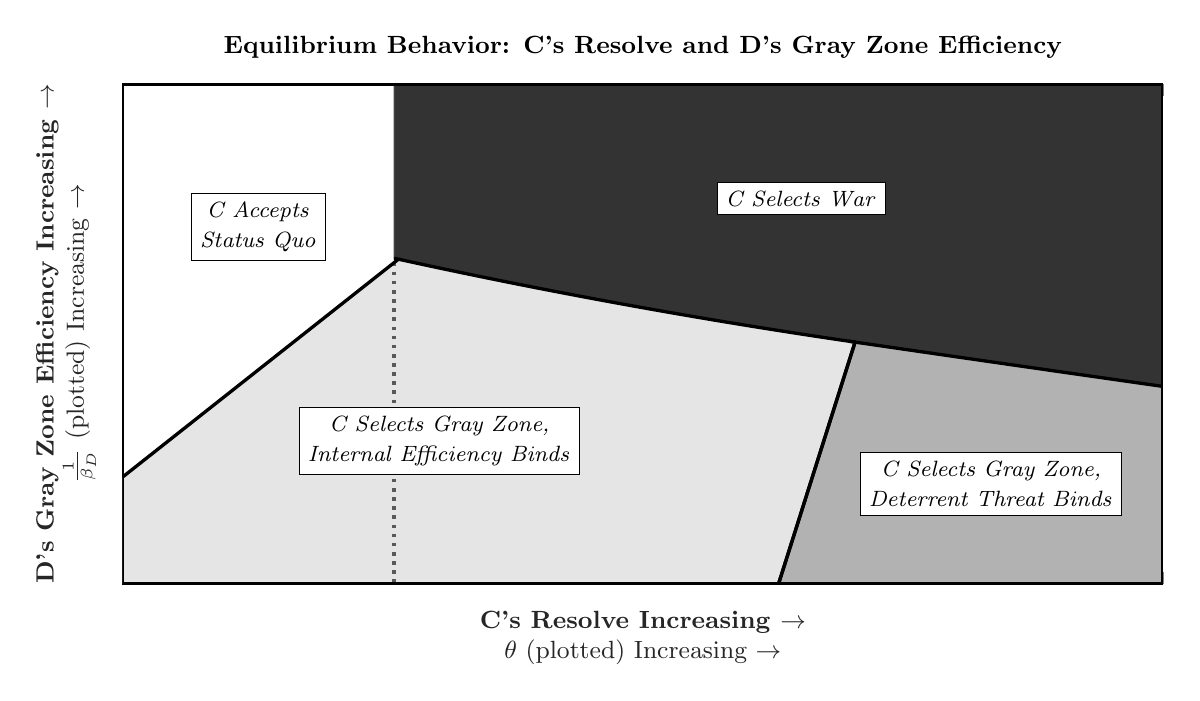
\begin{tikzpicture} 
    \small
    \begin{axis}[%
    width=5.2in,
    height=2.5in,
    at={(1.011in,0.642in)},
    scale only axis,
    xmin=1.285,
    xmax=1.4,
    xtick={1.285, 1.315, 1.4},
    xticklabels={{},{},{}},
    %$$U_{C}(status\;quo) = U_{C}(war) \;\;\;\;\;\;\;\;\;\;$
    xlabel style={font=\color{white!15!black},align=center},
    xlabel={\textbf{C's Resolve Increasing $\rightarrow$} \\ $\theta$ (plotted) Increasing $\rightarrow$},
    ymin=0.635,
    ymax=0.67,
    ytick={0.635, 0.67},
    yticklabels={{},{}},
    ylabel style={font=\color{white!15!black}, align=center},
    ylabel={\textbf{D's Gray Zone Efficiency Increasing $\rightarrow$} \\ $\frac{1}{\beta_D}$ (plotted) Increasing $\rightarrow$},
    axis background/.style={fill=white},
    title style={font=\bfseries},
    title={Equilibrium Behavior: C's Resolve and D's Gray Zone Efficiency},
    ]
    
     
    %\node[draw, align=center] at (.1925,1.2) {\footnotesize{\textit{Gray Zone,}} \\ \footnotesize{\textit{Unconstrained}}}; 
    
    
    
    %NEW ATTEMPT
    %WAR
    \draw [black!70!white, fill=black!80!white]
    %IEB -->DTB
    	(1.3155, 0.65775) -- (	1.315, 0.657804183	)	--
    (	1.316	,	0.657665653	)	--
    (	1.317	,	0.657528094	)	--
    (	1.318	,	0.657391502	)	--
    (	1.319	,	0.657255876	)	--
    (	1.32	,	0.657121212	)	--
    (	1.321	,	0.656987509	)	--
    (	1.322	,	0.656854766	)	--
    (	1.323	,	0.656722978	)	--
    (	1.324	,	0.656592145	)	--
    (	1.325	,	0.656462264	)	--
    (	1.326	,	0.656333333	)	--
    (	1.327	,	0.65620535	)	--
    (	1.328	,	0.656078313	)	--
    (	1.329	,	0.65595222	)	--
    (	1.33	,	0.655827068	)	--
    (	1.331	,	0.655702855	)	--
    (	1.332	,	0.65557958	)	--
    (	1.333	,	0.655457239	)	--
    (	1.334	,	0.655335832	)	--
    (	1.335	,	0.655215356	)	--
    (	1.336	,	0.655095808	)	--
    (	1.337	,	0.654977188	)	--
    (	1.338	,	0.654859492	)	--
    (	1.339	,	0.654742718	)	--
    (	1.34	,	0.654626866	)	--
    (	1.341	,	0.654511931	)	--
    (	1.342	,	0.654397914	)	--
    (	1.343	,	0.65428481	)	--
    (	1.344	,	0.654172619	)	--
    (	1.345	,	0.654061338	)	--
    (	1.346	,	0.653950966	)	--
    (	1.347	,	0.6538415	)	--
    (	1.348	,	0.653732938	)	--
    (	1.349	,	0.653625278	)	--
    (	1.35	,	0.653518519	)	--
    (	1.351	,	0.653412657	)	--
    (	1.352	,	0.653307692	)	--
    (	1.353	,	0.653203622	)	--
    (	1.354	,	0.653100443	)	--
    (	1.355	,	0.652998155	)	--
    (	1.356	,	0.652896755	)	--
    (	1.357	,	0.652796242	)	--
    (	1.358	,	0.652696613	)	--
    (	1.359	,	0.652597866	)	--
    (	1.36	,	0.6525	)	--
    (	1.361	,	0.652403012	)	--
    (	1.362	,	0.652306902	)	--
    (	1.363	,	0.652211665	)	--
    (	1.364	,	0.652117302	)	--
    (	1.365	,	0.65202381	)	--
    (	1.366	,	0.651931186	)	--
    %BREAK HERE
    (	1.365253968	,	0.652	)	--
    (	1.36633822	,	0.6519	)	--
    (	1.367423312	,	0.6518	)	--
    (	1.368509247	,	0.6517	)	--
    (	1.369596025	,	0.6516	)	--
    (	1.370683648	,	0.6515	)	--
    (	1.371772116	,	0.6514	)	--
    (	1.372861431	,	0.6513	)	--
    (	1.373951592	,	0.6512	)	--
    (	1.375042603	,	0.6511	)	--
    (	1.376134462	,	0.651	)	--
    (	1.377227172	,	0.6509	)	--
    (	1.378320734	,	0.6508	)	--
    (	1.379415148	,	0.6507	)	--
    (	1.380510415	,	0.6506	)	--
    (	1.381606537	,	0.6505	)	--
    (	1.382703514	,	0.6504	)	--
    (	1.383801348	,	0.6503	)	--
    (	1.38490004	,	0.6502	)	--
    (	1.38599959	,	0.6501	)	--
    (	1.3871	,	0.65	)	--
    (	1.388201271	,	0.6499	)	--
    (	1.389303403	,	0.6498	)	--
    (	1.390406398	,	0.6497	)	--
    (	1.391510256	,	0.6496	)	--
    (	1.39261498	,	0.6495	)	--
    (	1.393720569	,	0.6494	)	--
    (	1.394827026	,	0.6493	)	--
    (	1.39593435	,	0.6492	)	--
    (	1.397042543	,	0.6491	)	--
    (	1.398151606	,	0.649	)	--
    (	1.399261541	,	0.6489	)	--
    (	1.400372347	,	0.6488	)	--
    (	1.401484027	,	0.6487	)	--
    (	1.402596581	,	0.6486	)	--
    (	1.40371001	,	0.6485	)	--
    (	1.404824316	,	0.6484	)	--
    (	1.405939499	,	0.6483	)	--
    (	1.40705556	,	0.6482	)	--
    (	1.408172501	,	0.6481	)	--
    (	1.409290323	,	0.648	)	--
    %GOING UP NOW
    (1.4,0.65) -- (1.4,0.69) --(1.315,0.69) -- (1.315,0.65775);
    
    %SQO
    %\draw [black!70!white, fill=black!00!white](1.29,0.6425) -- (1.315,0.65775) -- 
    %	(1.315,0.69) -- (1.29,0.69) ;
    
    %GZ, DTB
    \draw [black!90!white, fill=black!30!white](1.3575, 0.635) -- (1.366	, 0.652) -- 
    	(	1.365253968	,	0.652	)	--
    (	1.36633822	,	0.6519	)	--
    (	1.367423312	,	0.6518	)	--
    (	1.368509247	,	0.6517	)	--
    (	1.369596025	,	0.6516	)	--
    (	1.370683648	,	0.6515	)	--
    (	1.371772116	,	0.6514	)	--
    (	1.372861431	,	0.6513	)	--
    (	1.373951592	,	0.6512	)	--
    (	1.375042603	,	0.6511	)	--
    (	1.376134462	,	0.651	)	--
    (	1.377227172	,	0.6509	)	--
    (	1.378320734	,	0.6508	)	--
    (	1.379415148	,	0.6507	)	--
    (	1.380510415	,	0.6506	)	--
    (	1.381606537	,	0.6505	)	--
    (	1.382703514	,	0.6504	)	--
    (	1.383801348	,	0.6503	)	--
    (	1.38490004	,	0.6502	)	--
    (	1.38599959	,	0.6501	)	--
    (	1.3871	,	0.65	)	--
    (	1.388201271	,	0.6499	)	--
    (	1.389303403	,	0.6498	)	--
    (	1.390406398	,	0.6497	)	--
    (	1.391510256	,	0.6496	)	--
    (	1.39261498	,	0.6495	)	--
    (	1.393720569	,	0.6494	)	--
    (	1.394827026	,	0.6493	)	--
    (	1.39593435	,	0.6492	)	--
    (	1.397042543	,	0.6491	)	--
    (	1.398151606	,	0.649	)	--
    (	1.399261541	,	0.6489	)	--
    (	1.400,	0.6488	)	--
    (1.4,0.635) ;
    
    %GZ IEB
    \draw [black!90!white, fill=black!10!white] (1.285, 0.635) -- (1.285, 0.6425) -- 
    	(1.3155, 0.65775) -- (	1.315, 0.657804183	)	--
    (	1.316	,	0.657665653	)	--
    (	1.317	,	0.657528094	)	--
    (	1.318	,	0.657391502	)	--
    (	1.319	,	0.657255876	)	--
    (	1.32	,	0.657121212	)	--
    (	1.321	,	0.656987509	)	--
    (	1.322	,	0.656854766	)	--
    (	1.323	,	0.656722978	)	--
    (	1.324	,	0.656592145	)	--
    (	1.325	,	0.656462264	)	--
    (	1.326	,	0.656333333	)	--
    (	1.327	,	0.65620535	)	--
    (	1.328	,	0.656078313	)	--
    (	1.329	,	0.65595222	)	--
    (	1.33	,	0.655827068	)	--
    (	1.331	,	0.655702855	)	--
    (	1.332	,	0.65557958	)	--
    (	1.333	,	0.655457239	)	--
    (	1.334	,	0.655335832	)	--
    (	1.335	,	0.655215356	)	--
    (	1.336	,	0.655095808	)	--
    (	1.337	,	0.654977188	)	--
    (	1.338	,	0.654859492	)	--
    (	1.339	,	0.654742718	)	--
    (	1.34	,	0.654626866	)	--
    (	1.341	,	0.654511931	)	--
    (	1.342	,	0.654397914	)	--
    (	1.343	,	0.65428481	)	--
    (	1.344	,	0.654172619	)	--
    (	1.345	,	0.654061338	)	--
    (	1.346	,	0.653950966	)	--
    (	1.347	,	0.6538415	)	--
    (	1.348	,	0.653732938	)	--
    (	1.349	,	0.653625278	)	--
    (	1.35	,	0.653518519	)	--
    (	1.351	,	0.653412657	)	--
    (	1.352	,	0.653307692	)	--
    (	1.353	,	0.653203622	)	--
    (	1.354	,	0.653100443	)	--
    (	1.355	,	0.652998155	)	--
    (	1.356	,	0.652896755	)	--
    (	1.357	,	0.652796242	)	--
    (	1.358	,	0.652696613	)	--
    (	1.359	,	0.652597866	)	--
    (	1.36	,	0.6525	)	--
    (	1.361	,	0.652403012	)	--
    (	1.362	,	0.652306902	)	--
    (	1.363	,	0.652211665	)	--
    (	1.364	,	0.652117302	)	--
    (	1.365	,	0.65202381	)	--
    (	1.366	,	0.651931186	)	--
    (1.3575,0.635) ;
    
    
    
    
    %OLD ATTEMPT
    
    %BEGIN DOTTED LINES
    
    \addplot [color=white!35!black, dotted, line width=1.3pt, forget plot]
      table[row sep=crcr]{%
    1.315 	0.6575\\
    1.315	0.647\\
    };
    
    \addplot [color=white!35!black, dotted, line width=1.3pt, forget plot]
      table[row sep=crcr]{%
    1.315	0.643\\
    1.315	0.635\\
    };
    
    
    %END DOTTED LINES
    
    
    
    
    %xmin=1.285,
    %xmax=1.4,
    %ymin=0.635,
    %ymax=0.67,
    \addplot [color=black, line width=1.2pt]
      table[row sep=crcr]{%
    1.285	0.635	\\
    1.285	0.67	\\
    };
    
    \addplot [color=black, line width=1.2pt]
      table[row sep=crcr]{%
    1.285	0.635	\\
    1.4	0.635	\\
    };
    
    \addplot [color=black, line width=1.2pt]
      table[row sep=crcr]{%
    1.285	0.67	\\
    1.4	0.67	\\
    };
    
    \addplot [color=black, line width=1.2pt]
      table[row sep=crcr]{%
    1.4	0.635	\\
    1.4	0.67	\\
    };
    
    
    
    \addplot [color=black, line width=1.2pt]
      table[row sep=crcr]{%
    1.3575	0.635	\\
    1.358	0.636	\\
    1.3585	0.637	\\
    1.359	0.638	\\
    1.3595	0.639	\\
    1.36	0.64	\\
    1.3605	0.641	\\
    1.361	0.642	\\
    1.3615	0.643	\\
    1.362	0.644	\\
    1.3625	0.645	\\
    1.363	0.646	\\
    1.3635	0.647	\\
    1.364	0.648	\\
    1.3645	0.649	\\
    1.365	0.65	\\
    1.3655	0.651	\\
    1.366	0.652	\\
    };
    
    
    
    %GZ CONSTRAINTS
    \addplot [color=black, line width=1.2pt]
      table[row sep=crcr]{%
    1.3575	0.635	\\
    1.358	0.636	\\
    1.3585	0.637	\\
    1.359	0.638	\\
    1.3595	0.639	\\
    1.36	0.64	\\
    1.3605	0.641	\\
    1.361	0.642	\\
    1.3615	0.643	\\
    1.362	0.644	\\
    1.3625	0.645	\\
    1.363	0.646	\\
    1.3635	0.647	\\
    1.364	0.648	\\
    1.3645	0.649	\\
    1.365	0.65	\\
    1.3655	0.651	\\
    1.366	0.652	\\
    };
    
    %GZ INTERIOR PEACE
    \addplot [color=black, line width=1.2pt, forget plot]
      table[row sep=crcr]{%
    1.285	0.6425	\\
    1.286	0.643	\\
    1.287	0.6435	\\
    1.288	0.644	\\
    1.289	0.6445	\\
    1.29	0.645	\\
    1.291	0.6455	\\
    1.292	0.646	\\
    1.293	0.6465	\\
    1.294	0.647	\\
    1.295	0.6475	\\
    1.296	0.648	\\
    1.297	0.6485	\\
    1.298	0.649	\\
    1.299	0.6495	\\
    1.3	0.65	\\
    1.301	0.6505	\\
    1.302	0.651	\\
    1.303	0.6515	\\
    1.304	0.652	\\
    1.305	0.6525	\\
    1.306	0.653	\\
    1.307	0.6535	\\
    1.308	0.654	\\
    1.309	0.6545	\\
    1.31	0.655	\\
    1.311	0.6555	\\
    1.312	0.656	\\
    1.313	0.6565	\\
    1.314	0.657	\\
    1.315	0.6575	\\
    1.3155	0.65775	\\
    };
    
    %GZ INTERIOR WAR
    \addplot [color=black, line width=1.2pt, forget plot]
      table[row sep=crcr]{%
    1.315	0.657804183	\\
    1.316	0.657665653	\\
    1.317	0.657528094	\\
    1.318	0.657391502	\\
    1.319	0.657255876	\\
    1.32	0.657121212	\\
    1.321	0.656987509	\\
    1.322	0.656854766	\\
    1.323	0.656722978	\\
    1.324	0.656592145	\\
    1.325	0.656462264	\\
    1.326	0.656333333	\\
    1.327	0.65620535	\\
    1.328	0.656078313	\\
    1.329	0.65595222	\\
    1.33	0.655827068	\\
    1.331	0.655702855	\\
    1.332	0.65557958	\\
    1.333	0.655457239	\\
    1.334	0.655335832	\\
    1.335	0.655215356	\\
    1.336	0.655095808	\\
    1.337	0.654977188	\\
    1.338	0.654859492	\\
    1.339	0.654742718	\\
    1.34	0.654626866	\\
    1.341	0.654511931	\\
    1.342	0.654397914	\\
    1.343	0.65428481	\\
    1.344	0.654172619	\\
    1.345	0.654061338	\\
    1.346	0.653950966	\\
    1.347	0.6538415	\\
    1.348	0.653732938	\\
    1.349	0.653625278	\\
    1.35	0.653518519	\\
    1.351	0.653412657	\\
    1.352	0.653307692	\\
    1.353	0.653203622	\\
    1.354	0.653100443	\\
    1.355	0.652998155	\\
    1.356	0.652896755	\\
    1.357	0.652796242	\\
    1.358	0.652696613	\\
    1.359	0.652597866	\\
    1.36	0.6525	\\
    1.361	0.652403012	\\
    1.362	0.652306902	\\
    1.363	0.652211665	\\
    1.364	0.652117302	\\
    1.365	0.65202381	\\
    1.366	0.651931186	\\
    };
    
    %GZ External WAR
    \addplot [color=black, line width=1.2pt, forget plot]
      table[row sep=crcr]{%
    1.409290323	0.648	\\
    1.408172501	0.6481	\\
    1.40705556	0.6482	\\
    1.405939499	0.6483	\\
    1.404824316	0.6484	\\
    1.40371001	0.6485	\\
    1.402596581	0.6486	\\
    1.401484027	0.6487	\\
    1.400372347	0.6488	\\
    1.399261541	0.6489	\\
    1.398151606	0.649	\\
    1.397042543	0.6491	\\
    1.39593435	0.6492	\\
    1.394827026	0.6493	\\
    1.393720569	0.6494	\\
    1.39261498	0.6495	\\
    1.391510256	0.6496	\\
    1.390406398	0.6497	\\
    1.389303403	0.6498	\\
    1.388201271	0.6499	\\
    1.3871	0.65	\\
    1.38599959	0.6501	\\
    1.38490004	0.6502	\\
    1.383801348	0.6503	\\
    1.382703514	0.6504	\\
    1.381606537	0.6505	\\
    1.380510415	0.6506	\\
    1.379415148	0.6507	\\
    1.378320734	0.6508	\\
    1.377227172	0.6509	\\
    1.376134462	0.651	\\
    1.375042603	0.6511	\\
    1.373951592	0.6512	\\
    1.372861431	0.6513	\\
    1.371772116	0.6514	\\
    1.370683648	0.6515	\\
    1.369596025	0.6516	\\
    1.368509247	0.6517	\\
    1.367423312	0.6518	\\
    1.36633822	0.6519	\\
    1.365253968	0.652	\\
    };
    
      %   \node at (1.3,0.502)  [circle,scale=0.7,minimum size=0.5pt,draw,fill=black!100] {};
      %  \node at (1.3,0.65)  [circle,scale=0.7,draw,fill=black!0] {};
    \node[draw, fill=white, align=center] at (1.3,0.66) {\footnotesize{\textit{C Accepts}} \\ \footnotesize{\textit{Status Quo}}};
    \node[draw, fill=white, align=center] at (1.32,0.645) {\footnotesize{\textit{C Selects Gray Zone,}} \\ \footnotesize{\textit{Internal Efficiency Binds}}}; 
    \node[draw, fill=white, align=center] at (1.381,0.642) {\footnotesize{\textit{C Selects Gray Zone,}} \\ \footnotesize{\textit{Deterrent Threat Binds}}}; 
    \node[draw, fill=white, align=center] at (1.36,0.662) {\footnotesize{\textit{C Selects War}}};
    
    \end{axis}
    \end{tikzpicture}
    
    \caption{Equilibrium behavior as C's resolve and D's gray zone efficiency varies}
    \floatnote{C's resolve $\theta$ and the inverse D's gray zone efficiency $\frac{1}{\beta_D}$ are plotted. The dashed line is on the $\theta$ value where $\theta=\frac{\kappa_{C}}{\rho_W-\rho_0}$, or where C is indifferent between initially accepting the status quo and going to war. 
    %The x-axis endpoints are $\theta=1.285$ and $\theta=1.4$. The y-axis endpoints are $\frac{1}{\beta_D}=0.635$ and $\frac{1}{\beta_D}=0.67$. 
    The parameters are $\rho_0=0$, $\rho_W=0.5$, $\beta_C=1$, $\kappa_{C}=0.53$, and $\kappa_D=0.1$.}
    \label{fig:equilibrium}
    \end{figure}

Figure \ref{fig:equilibrium} details this logic. On the x-axis, we plot C's resolve. On the y-axis, we plot D's costs of gray zone conflict. Each region of the graph is an equilibrium type. For example, ``C Selects Gray Zone, No Deterrent Threat'' is described in Case 2.C. in Proposition 1. The dotted line represents the cut-point where, to the left, C prefers the status quo to war, and to the right, C prefers war to the status quo. Figure \ref{fig:equilibrium} conveys that D does not always benefit by increasing its ability to resist gray zone conflict. Consider a point in the ``C Selects Gray Zone, Internal Efficiency Binds'' region that is to the left of the dotted line. Here if D's gray zone efficiency increases, then after some point, C will forgo gray zone conflict altogether and accept the status quo. In this circumstance, C has a low-enough resolve that, with sufficient pressure, C can be deterred from all forms of conflict. However, consider now a point in the same equilibrium region, but to the right of the dotted line. If $\beta_{D}$ increases above some point, C will choose war. In this circumstance, C is resolved enough that as D gets too good at countering gray zone conflict, C will opt into war. 

\textbf{\textit{Observation 4:}}\textit{ Decreases in D's gray zone costs ($\beta_{D}$) can lead to less or more conflict.}

There is an alternate interpretation; $\beta_{D}$ could be influenced by the defender's prior, un-modeled moves in the game that set up current gray zone operations. For example, if the defender aggressively pursued counterinsurgency operations against foreign-backed rebels before this game began, the defender could be in a position to pursue aggressive gray zone conflict within the game. This interpretation illustrates how it is not just latent, exogenous costs that influence the challenger's activity, but rather war can resuly from the defender behaving too aggressively in prior actions against a highly resolved challenger. 

This final interpretation has important policy consequences. Even if most actors are assumed to harbor challenger ambitions \citep{schweller_neorealismstatusquo_1996}, would-be defenders still face a security-like dilemma in shaping how aggression is expressed. In the security dilemma, the outcome of a ``threat'' from the target is a function of whether or not a challenger is resolved. Conflict short of war complicates this picture because gray zone behavior by a highly resolved challenger and by a marginally-resolved challenger may be observationally indistinguishable. And yet, the consequence of the defender threatening to escalate within gray zone conflict vastly differs. The new U.S. Cyber Command doctrine of ``persistent engagement'' aims to establish dominance in strategic competition short of war through proactively ``defending forward,'' but its very success could become the trigger for inadvertent escalation \citep{healey_escalationinversionother_2020}.

While we have focused on Russian gray zone conflict, we expect our theory to apply to conflict among capable powers more generally. Chinese incursions in the South China Sea offer another potential test. China’s use of ``little blue men'' suggests that opportunism and restraint are both enabling and constraining Chinese foreign policy. That is, Beijing appears to fear that the use of more intense military operations risks provoking a Western response that both sides hope to avoid \citep{zhang_cautiousbullyreputation_2019}. Focusing on the credibility of deterrence rather than the novelty of means used for gray-zone conflict can also help to evaluate proper policy responses \citep{green_counteringcoercionmaritime_2017}. Confronted with gray zone provocations by capable actors like Russia, China, and Iran, the United States would be well advised to reinforce its strengths while avoiding over-extension.

\section{Every Silver Lining's Got a Touch of Gray}
Gray zone conflict occurs when capable actors intentionally limit the intensity or capacity of aggression and refrain from escalation. Deterrence shapes the way that conflict emerges, but it may not suppress conflict altogether. The good news is that gray zone conflict is symptomatic of deterrence success. The bad news is that gray zone conflict probes the threshold of deterrence effectiveness. We expect conflict severity to be greater wherever there are questions about the willingness or ability of defenders to respond forcefully. An adversary is seldom passive. There will always be attempts at end-runs or push-back, even when deterrence is credible. It is thus important to think carefully before overextending commitments where credibility is in doubt. 

Just as there is a gray zone between war and peace, the distinction between effective and ineffective deterrence is also fuzzy. We have introduced the notion of a deterrence gradient, a straightforward extrapolation from the military loss of strength gradient, to describe credible deterrence as a continuous variable. Wherever deterrence is credible, or the challenger's resolve is low, challengers can be expected to exercise restraint as they probe to see what they can get away with. Wherever deterrence is not credible or challengers are highly resolved, however, a challenger must be more emboldened to use whatever means they have at their disposal to meet their objectives, limited only by internal efficiency constraints. The challenge lies between these extremes, where the variable threshold of credibility creates a policy arena for limited conflict, and where it can be difficult to distinguish efficiency motivations from risk sensitivity. Doubling down on deterrence can mitigate conflict in the latter case but provoke escalation in the former.

We have used the same cases that have raised alarms about the dangers of gray zone conflict—--Russian incursions in Georgia and Ukraine and cyber campaigns targeting many other countries—--to suggest the validity of an alternative explanation. The evidence suggests that Russia systematically reduces the intensity of its interventions along the deterrence gradient, employing a greater variety of means with more lethal intensity where deterrence is weakest but conducting only ambiguous information operations where deterrence is most robust. The conventional wisdom is right that Russian interventions are paradigmatic exemplars of gray zone conflict, but it is wrong about Russian motivations and the effectiveness of these operations. Revisionist powers such as Russia have not discovered a secret formula or novel tools destined to destabilize Western democracies or undermine NATO's deterrence posture. Rather it acts opportunistically as circumstances enable it to hassle adversaries and their clients without, however, risking a costly military confrontation that Moscow does not want. The flip side of this logic, however, is that Russia is willing to call NATO’s bluffs in cases where it can reasonably expect that NATO is unwilling to intervene. In Georgia, and even more so in Chechnya, Russian willingness to prioritize effectiveness at the price of efficiency is clear.

This argument has implications for the debate over NATO expansion after the Cold War \citep{shifrinson_dealnodeal_2016}. When expansion is posed in starkly binary terms, it can be seen as either a stabilizing force for Europe or an irresponsible provocation of legitimate Russian security interests fueled by liberal expansionism \citep{mcfaul_faultypowers_2014, mearsheimer_whyukrainecrisis_2014}. If deterrence and conflict are continuous variables, however, then the real question is not simply whether NATO should or should not have expanded its security guarantees, but how far. One might thus argue that the first round of expansion to include the Eastern-Central countries (Poland, Hungary, Czech Republic) under the NATO umbrella helped to stabilize an historically conflict-prone portion of Europe. After the fall of the Soviet Union and during a period of military and economic weakness, moreover, Russia was grudgingly willing to accept a reduction in its European influence. One might also debate whether later rounds which brought in Baltic and Balkan countries made sense in whole or part. This is not the place to debate this history. We merely wish to point out that the alternative perspectives of NATO provocation and Russian aggression are better conceived of as context specific variables rather than absolute qualities of either actor. The right question is not whether NATO should have expanded, but how far.

Just as deterrence varies along the gradient, the contours of the gradient can shift over time. When NATO’s relative power was increasing, expansion was defensible. If NATO’s relative power decreases for whatever reason, then retrenchment makes more sense. Conversely, declining Russian relative power may enable NATO to bolster the line, rendering today’s gray zone provocations more prohibitive tomorrow. Gray zone conflict allows keen observers to map the contours of the deterrence gradient, especially in areas where the ``defender'' has overreached its ability or will to respond. As information about the gradient is revealed, actors can take steps to shore up defenses and reassess priorities. Russia has advertised its willingness to interfere in elections, distort public debate, mobilize nationalist movements, and engage in other provocations. This in turn has led Western governments and publics to heighten awareness, increased vigilance, renewed defenses, and deterrence postures. Much as the shooting down of the Malaysian Airlines flight over Donetsk led both to renewed debate within NATO about intervention and to greater restraint in Moscow, so too the lowering of credible escalation thresholds can help to contain risk-averse opportunists. Just as gray zone conflict is symptomatic of deterrence success, the increasing incidence of Russian provocation may be symptomatic of a closing window for its effectiveness, such as it is.

The very fact that an adversary opts to engage in limited conflict suggests both vulnerabilities and opportunities. Instead of worrying that Russia is outwitting the West, we should instead realize that NATO has already blocked Russia from wielding even greater influence. The implicit general deterrence posture of NATO and the United States has arguably succeeded in keeping more extreme forms of Russian aggression in check. The unfortunate fact remains, however, that a simple remedy for gray zone conflict does not exist, because there is always some uncertainty about the precise contours of the deterrence gradient. We may be able to choose how our adversary confronts us, but not whether. Deterrence is not an on/off switch, but a rheostat, providing a range of causes and variable effects. Gray zone conflict is then not deterrence failure but a modest kind of success. 

\bibliography{GrayZone.bib}

\end{document}